%%%%%%%%%%%%%%%%%%%%%%%%%%%%%%%%%%%%%%%%%
% The Legrand Orange Book
% LaTeX Template
% Version 1.0 (25/3/13)
%
% This template has been downloaded from:
% http://www.LaTeXTemplates.com
%
% Original author:
% Mathias Legrand (legrand.mathias@gmail.com)
%
% License:
% CC BY-NC-SA 3.0 (http://creativecommons.org/licenses/by-nc-sa/3.0/)
%
% Compiling this template:
% This template uses biber for its bibliography and makeindex for its index.
% This means that to update the bibliography and index in this template you
% will need to run the following sequence of commands in the template
% directory:
%
% 1) pdflatex main
% 2) makeindex main.idx -s StyleInd.ist
% 3) biber main
% 4) pdflatex main
%
% This template also uses a number of packages which may need to be
% updated to the newest versions for the template to compile. It is strongly
% recommended you update your LaTeX distribution if you have any
% compilation errors.
%
% Important note:
% Chapter heading images should have a 2:1 width:height ratio,
% e.g. 920px width and 460px height.
%
%%%%%%%%%%%%%%%%%%%%%%%%%%%%%%%%%%%%%%%%%

%----------------------------------------------------------------------------------------
%	PACKAGES AND OTHER DOCUMENT CONFIGURATIONS
%----------------------------------------------------------------------------------------

\documentclass[11pt,fleqn]{book} % Default font size and left-justified equations

\usepackage[top=3cm,bottom=3cm,left=3.2cm,right=3.2cm,headsep=10pt,a4paper]{geometry} % Page margins

\usepackage{xcolor} % Required for specifying colors by name
\definecolor{ocre}{RGB}{243,102,25} % Define the orange color used for highlighting throughout the book

% Font Settings
\usepackage{avant} % Use the Avantgarde font for headings
%\usepackage{times} % Use the Times font for headings
\usepackage{mathptmx} % Use the Adobe Times Roman as the default text font together with math symbols from the Sym­bol, Chancery and Com­puter Modern fonts
\usepackage{microtype} % Slightly tweak font spacing for aesthetics
\usepackage[utf8]{inputenc} % Required for including letters with accents
\usepackage[T1]{fontenc} % Use 8-bit encoding that has 256 glyphs

% Bibliography
\usepackage[style=alphabetic,sorting=nyt,sortcites=true,autopunct=true,babel=hyphen,hyperref=true,abbreviate=false,backref=true,backend=biber]{biblatex}
\addbibresource{bibliography.bib} % BibTeX bibliography file
\defbibheading{bibempty}{}

% Index
\usepackage{calc} % For simpler calculation - used for spacing the index letter headings correctly
\usepackage{makeidx} % Required to make an index
\makeindex % Tells LaTeX to create the files required for indexing

% AWH - Code/file listings
\usepackage{color}
\usepackage{listings}
\lstset{ %
%language=C++,                % choose the language of the code
basicstyle=\footnotesize,       % the size of the fonts that are used for the code
numbers=left,                   % where to put the line-numbers
numberstyle=\footnotesize,      % the size of the fonts that are used for the line-numbers
stepnumber=1,                   % the step between two line-numbers. If it is 1 each line will be numbered
numbersep=5pt,                  % how far the line-numbers are from the code
backgroundcolor=\color{white},  % choose the background color. You must add \usepackage{color}
showspaces=false,               % show spaces adding particular underscores
showstringspaces=false,         % underline spaces within strings
showtabs=false,                 % show tabs within strings adding particular underscores
frame=single,           % adds a frame around the code
tabsize=2,          % sets default tabsize to 2 spaces
captionpos=b,           % sets the caption-position to bottom
breaklines=true,        % sets automatic line breaking
breakatwhitespace=false,    % sets if automatic breaks should only happen at whitespace
%title=\lstname,
escapeinside={\%*}{*)}          % if you want to add a comment within your code
}

\RequirePackage[framemethod=default]{mdframed}

% AWH - Attention box
\newenvironment{updateWarn}{\begin{cBox}\begin{tabular}{l l}{\begin{minipage}[c]{1cm}
\includegraphics[scale=0.05]{Boris_Bone.png}\end{minipage}}&\begin{minipage}[c]{12cm}}{\end{minipage}\end{tabular}\end{cBox}}

%AWH - Command box
\newmdenv[skipabove=7pt,
skipbelow=7pt,
backgroundcolor=black!5,
linecolor=ocre,
innerleftmargin=5pt,
innerrightmargin=5pt,
innertopmargin=5pt,
leftmargin=0cm,
rightmargin=0cm,
innerbottommargin=5pt]{cmdBox}
\newenvironment{commandBox}{\begin{cmdBox}}{\end{cmdBox}}

\newcommand{\ignore}[1]{}
%----------------------------------------------------------------------------------------

%----------------------------------------------------------------------------------------
%	VARIOUS REQUIRED PACKAGES
%----------------------------------------------------------------------------------------

\usepackage{titlesec} % Allows customization of titles

\usepackage{graphicx} % Required for including pictures
\graphicspath{{./Pictures/}} % Specifies the directory where pictures are stored

\usepackage{lipsum} % Inserts dummy text

\usepackage{tikz} % Required for drawing custom shapes

\usepackage[english]{babel} % English language/hyphenation

\usepackage{enumitem} % Customize lists
\setlist{nolistsep} % Reduce spacing between bullet points and numbered lists

\usepackage{booktabs} % Required for nicer horizontal rules in tables

\usepackage{eso-pic} % Required for specifying an image background in the title page

%----------------------------------------------------------------------------------------
%	MAIN TABLE OF CONTENTS
%----------------------------------------------------------------------------------------

\usepackage{titletoc} % Required for manipulating the table of contents

\contentsmargin{0cm} % Removes the default margin
% Chapter text styling
\titlecontents{chapter}[1.25cm] % Indentation
{\addvspace{15pt}\large\sffamily\bfseries} % Spacing and font options for chapters
{\color{ocre!60}\contentslabel[\Large\thecontentslabel]{1.25cm}\color{ocre}} % Chapter number
{}  
{\color{ocre!60}\normalsize\sffamily\bfseries\;\titlerule*[.5pc]{.}\;\thecontentspage} % Page number
% Section text styling
\titlecontents{section}[1.25cm] % Indentation
{\addvspace{5pt}\sffamily\bfseries} % Spacing and font options for sections
{\contentslabel[\thecontentslabel]{1.25cm}} % Section number
{}
{\sffamily\hfill\color{black}\thecontentspage} % Page number
[]
% Subsection text styling
\titlecontents{subsection}[1.25cm] % Indentation
{\addvspace{1pt}\sffamily\small} % Spacing and font options for subsections
{\contentslabel[\thecontentslabel]{1.25cm}} % Subsection number
{}
{\sffamily\;\titlerule*[.5pc]{.}\;\thecontentspage} % Page number
[] 

%----------------------------------------------------------------------------------------
%	MINI TABLE OF CONTENTS IN CHAPTER HEADS
%----------------------------------------------------------------------------------------

% Section text styling
\titlecontents{lsection}[0em] % Indendating
{\footnotesize\sffamily} % Font settings
{}
{}
{}

% Subsection text styling
\titlecontents{lsubsection}[.5em] % Indentation
{\normalfont\footnotesize\sffamily} % Font settings
{}
{}
{}
 
%----------------------------------------------------------------------------------------
%	PAGE HEADERS
%----------------------------------------------------------------------------------------

\usepackage{fancyhdr} % Required for header and footer configuration

\pagestyle{fancy}
\renewcommand{\chaptermark}[1]{\markboth{\sffamily\normalsize\bfseries #1}{}} % Chapter text font settings
\renewcommand{\sectionmark}[1]{\markright{\sffamily\normalsize\thesection\hspace{5pt}#1}{}} % Section text font settings
\fancyhf{} \fancyhead[LE,RO]{\sffamily\normalsize\thepage} % Font setting for the page number in the header
\fancyhead[LO]{\rightmark} % Print the nearest section name on the left side of odd pages
\fancyhead[RE]{\leftmark} % Print the current chapter name on the right side of even pages
\renewcommand{\headrulewidth}{0.5pt} % Width of the rule under the header
\addtolength{\headheight}{2.5pt} % Increase the spacing around the header slightly
\renewcommand{\footrulewidth}{0pt} % Removes the rule in the footer
\fancypagestyle{plain}{\fancyhead{}\renewcommand{\headrulewidth}{0pt}} % Style for when a plain pagestyle is specified

% Removes the header from odd empty pages at the end of chapters
\makeatletter
\renewcommand{\cleardoublepage}{
\clearpage\ifodd\c@page\else
\hbox{}
\vspace*{\fill}
\thispagestyle{empty}
\newpage
\fi}

%----------------------------------------------------------------------------------------
%	THEOREM STYLES
%----------------------------------------------------------------------------------------

\usepackage{amsmath,amsfonts,amssymb,amsthm} % For including math equations, theorems, symbols, etc

\newcommand{\intoo}[2]{\mathopen{]}#1\,;#2\mathclose{[}}
\newcommand{\ud}{\mathop{\mathrm{{}d}}\mathopen{}}
\newcommand{\intff}[2]{\mathopen{[}#1\,;#2\mathclose{]}}
\newtheorem{notation}{Notation}[chapter]

\newtheoremstyle{ocrenum} % Theorem style name
{7pt} % Space above
{7pt} % Space below
{\normalfont} % Body font
{} % Indent amount
{\small\bf\sffamily\color{ocre}} % Theorem head font
{\;\;} % Punctuation after theorem head
{0.25em} % Space after theorem head
{\small\sffamily\color{ocre}\thmname{#1}\thmnumber{\@ifnotempty{#1}{ }\@upn{#2}} % Theorem text (e.g. Theorem 2.1)
\thmnote{\ {\the\thm@notefont\sffamily\bfseries\color{black}--- #3.}}} % Optional theorem note
\renewcommand{\qedsymbol}{$\blacksquare$} % Optional qed square

\newtheoremstyle{blacknumex} % Theorem style name
{7pt} % Space above
{7pt} % Space below
{\normalfont} % Body font
{} % Indent amount
{\small\bf\sffamily} % Theorem head font
{\;\;} % Punctuation after theorem head
{0.25em} % Space after theorem head
{\small\sffamily{\tiny\ensuremath{\blacksquare}}\ \thmname{#1}\thmnumber{\@ifnotempty{#1}{ }\@upn{#2}} % Theorem text (e.g. Theorem 2.1)
\thmnote{\ {\the\thm@notefont\sffamily\bfseries--- #3.}}} % Optional theorem note

\newtheoremstyle{blacknum} % Theorem style name
{7pt} % Space above
{7pt} % Space below
{\normalfont} % Body font
{} % Indent amount
{\small\bf\sffamily} % Theorem head font
{\;\;} % Punctuation after theorem head
{0.25em} % Space after theorem head
{\small\sffamily\thmname{#1}\thmnumber{\@ifnotempty{#1}{ }\@upn{#2}} % Theorem text (e.g. Theorem 2.1)
\thmnote{\ {\the\thm@notefont\sffamily\bfseries--- #3.}}} % Optional theorem note
\makeatother

% Defines the theorem text style for each type of theorem to one of the three styles above
\theoremstyle{ocrenum}
\newtheorem{theoremeT}{Theorem}[chapter]
\newtheorem{proposition}{Proposition}[chapter]
\newtheorem{problem}{Problem}[chapter]
\newtheorem{exerciseT}{Exercise}[chapter]
\theoremstyle{blacknumex}
\newtheorem{exampleT}{Example}[chapter]
\theoremstyle{blacknum}
\newtheorem{vocabulary}{Vocabulary}[chapter]
\newtheorem{definitionT}{Definition}[chapter]
\newtheorem{corollaryT}{Corollary}[chapter]

%----------------------------------------------------------------------------------------
%	DEFINITION OF COLORED BOXES
%----------------------------------------------------------------------------------------

\RequirePackage[framemethod=default]{mdframed} % Required for creating the theorem, definition, exercise and corollary boxes

% Theorem box
\newmdenv[skipabove=7pt,
skipbelow=7pt,
backgroundcolor=black!5,
linecolor=ocre,
innerleftmargin=5pt,
innerrightmargin=5pt,
innertopmargin=5pt,
leftmargin=0cm,
rightmargin=0cm,
innerbottommargin=5pt]{tBox}

% Exercise box	  
\newmdenv[skipabove=7pt,
skipbelow=7pt,
rightline=false,
leftline=true,
topline=false,
bottomline=false,
backgroundcolor=ocre!10,
linecolor=ocre,
innerleftmargin=5pt,
innerrightmargin=5pt,
innertopmargin=5pt,
innerbottommargin=5pt,
leftmargin=0cm,
rightmargin=0cm,
linewidth=4pt]{eBox}	

% Definition box
\newmdenv[skipabove=10pt,
skipbelow=10pt,
rightline=false,
leftline=true,
topline=false,
bottomline=false,
linecolor=ocre,
innerleftmargin=5pt,
innerrightmargin=5pt,
innertopmargin=0pt,
leftmargin=0cm,
rightmargin=0cm,
linewidth=4pt,
innerbottommargin=0pt]{dBox}	

% Corollary box
\newmdenv[skipabove=7pt,
skipbelow=7pt,
rightline=false,
leftline=true,
topline=false,
bottomline=false,
linecolor=gray,
backgroundcolor=black!5,
innerleftmargin=5pt,
innerrightmargin=5pt,
innertopmargin=5pt,
leftmargin=0cm,
rightmargin=0cm,
linewidth=4pt,
innerbottommargin=5pt]{cBox}				  
		  

% Creates an environment for each type of theorem and assigns it a theorem text style from the "Theorem Styles" section above and a colored box from above
\newenvironment{theorem}{\begin{tBox}\begin{theoremeT}}{\end{theoremeT}\end{tBox}}
\newenvironment{exercise}{\begin{eBox}\begin{exerciseT}}{\hfill{\color{ocre}\tiny\ensuremath{\blacksquare}}\end{exerciseT}\end{eBox}}				  
\newenvironment{definition}{\begin{dBox}\begin{definitionT}}{\end{definitionT}\end{dBox}}	
\newenvironment{example}{\begin{exampleT}}{\hfill{\tiny\ensuremath{\blacksquare}}\end{exampleT}}		
\newenvironment{corollary}{\begin{cBox}\begin{corollaryT}}{\end{corollaryT}\end{cBox}}	

%----------------------------------------------------------------------------------------
%	REMARK ENVIRONMENT
%----------------------------------------------------------------------------------------

\newenvironment{remark}{\par\vskip10pt\small % Vertical white space above the remark and smaller font size
\begin{list}{}{
\leftmargin=35pt % Indentation on the left
\rightmargin=25pt}\item\ignorespaces % Indentation on the right
\makebox[-2.5pt]{\begin{tikzpicture}[overlay]
\node[draw=ocre!60,line width=1pt,circle,fill=ocre!25,font=\sffamily\bfseries,inner sep=2pt,outer sep=0pt] at (-15pt,0pt){\textcolor{ocre}{R}};\end{tikzpicture}} % Orange R in a circle
\advance\baselineskip -1pt}{\end{list}\vskip5pt} % Tighter line spacing and white space after remark

%----------------------------------------------------------------------------------------
%	SECTION NUMBERING IN THE MARGIN
%----------------------------------------------------------------------------------------

\makeatletter
\renewcommand{\@seccntformat}[1]{\llap{\textcolor{ocre}{\csname the#1\endcsname}\hspace{1em}}}                    
\renewcommand{\section}{\@startsection{section}{1}{\z@}
{-4ex \@plus -1ex \@minus -.4ex}
{1ex \@plus.2ex }
{\normalfont\large\sffamily\bfseries}}
\renewcommand{\subsection}{\@startsection {subsection}{2}{\z@}
{-3ex \@plus -0.1ex \@minus -.4ex}
{0.5ex \@plus.2ex }
{\normalfont\sffamily\bfseries}}
\renewcommand{\subsubsection}{\@startsection {subsubsection}{3}{\z@}
{-2ex \@plus -0.1ex \@minus -.2ex}
{0.2ex \@plus.2ex }
{\normalfont\small\sffamily\bfseries}}                        
\renewcommand\paragraph{\@startsection{paragraph}{4}{\z@}
{-2ex \@plus-.2ex \@minus .2ex}
{0.1ex}
{\normalfont\small\sffamily\bfseries}}

%----------------------------------------------------------------------------------------
%	CHAPTER HEADINGS
%----------------------------------------------------------------------------------------

\newcommand{\thechapterimage}{}
\newcommand{\chapterimage}[1]{\renewcommand{\thechapterimage}{#1}}
\def\thechapter{\arabic{chapter}}
\def\@makechapterhead#1{
\thispagestyle{empty}
{\centering \normalfont\sffamily
\ifnum \c@secnumdepth >\m@ne
\if@mainmatter
\startcontents
\begin{tikzpicture}[remember picture,overlay]
\node at (current page.north west)
{\begin{tikzpicture}[remember picture,overlay]

\node[anchor=north west] at (-4pt,4pt) {\includegraphics[width=\paperwidth]{\thechapterimage}};

%Commenting the 3 lines below removes the small contents box in the chapter heading
\draw[fill=white,opacity=.6] (1cm,0) rectangle (8cm,-7cm);
\node[anchor=north west] at (1cm,.25cm) {\parbox[t][8cm][t]{6.5cm}{\huge\bfseries\flushleft \printcontents{l}{1}{\setcounter{tocdepth}{2}}}};

\draw[anchor=west] (5cm,-9cm) node [rounded corners=25pt,fill=white,opacity=.7,inner sep=15.5pt]{\huge\sffamily\bfseries\textcolor{black}{\vphantom{plPQq}\makebox[22cm]{}}};
\draw[anchor=west] (5cm,-9cm) node [rounded corners=25pt,draw=ocre,line width=2pt,inner sep=15pt]{\huge\sffamily\bfseries\textcolor{black}{\thechapter\ ---\ #1\vphantom{plPQq}\makebox[22cm]{}}};
\end{tikzpicture}};
\end{tikzpicture}}\par\vspace*{230\p@}
}
\def\@makeschapterhead#1{
\thispagestyle{empty}
{\centering \normalfont\sffamily
\ifnum \c@secnumdepth >\m@ne
\if@mainmatter
\startcontents
\begin{tikzpicture}[remember picture,overlay]
\node at (current page.north west)
{\begin{tikzpicture}[remember picture,overlay]
\node[anchor=north west] at (-4pt,4pt) {\includegraphics[width=\paperwidth]{\thechapterimage}};
\draw[anchor=west] (5cm,-9cm) node [rounded corners=25pt,fill=white,opacity=.7,inner sep=15.5pt]{\huge\sffamily\bfseries\textcolor{black}{\vphantom{plPQq}\makebox[22cm]{}}};
\draw[anchor=west] (5cm,-9cm) node [rounded corners=25pt,draw=ocre,line width=2pt,inner sep=15pt]{\huge\sffamily\bfseries\textcolor{black}{#1\vphantom{plPQq}\makebox[22cm]{}}};
\end{tikzpicture}};
\end{tikzpicture}}\par\vspace*{230\p@}
}
\makeatother % Insert the commands.tex file which contains the majority of the structure behind the template

\begin{document}

%----------------------------------------------------------------------------------------
%	TITLE PAGE
%----------------------------------------------------------------------------------------

\begingroup
\thispagestyle{empty}
\AddToShipoutPicture*{\put(6,5){
\includegraphics[scale=1]{background.pdf}}} % Image background
%\AddToShipoutPicture*{\put(0,0){
%  \parbox[b][\paperheight]{\paperwidth}{
%    \hspace{-0.2in}
\includegraphics[width=29.7cm,keepaspectratio,angle=90,origin=c]{working/background.jpg}
%    \vfill}}}
\centering
\vspace*{9cm}
%\par\normalfont\fontsize{35}{35}\sffamily\selectfont
\par\normalfont\fontsize{35}{35}\sffamily\selectfont
BeagleSNES v0.6 User and Developer Guide\par % Book title
\vspace*{1cm}
{\Huge Andrew Henderson}\par % Author name
{\Huge www.beaglesnes.org}\par % Author name
\endgroup

%----------------------------------------------------------------------------------------
%	COPYRIGHT PAGE
%----------------------------------------------------------------------------------------

\newpage
~\vfill
\thispagestyle{empty}

\noindent Copyright \copyright\ 2014 Andrew Henderson (hendersa@icculus.org)\\ % Copyright notice

%\noindent \textsc{Published by Publisher}\\ % Publisher

\noindent \textsc{www.beaglesnes.org}\\ % URL

\noindent Licensed under the Creative Commons Attribution-NonCommercial 3.0 Unported License (the ``License''). You may not use this file except in compliance with the License. You may obtain a copy of the License at \url{http://creativecommons.org/licenses/by-nc/3.0}. Unless required by applicable law or agreed to in writing, software distributed under the License is distributed on an \textsc{``AS IS'' BASIS, WITHOUT WARRANTIES OR CONDITIONS OF ANY KIND}, either express or implied. See the License for the specific language governing permissions and limitations under the License.\\ % License information

%\noindent \textit{First printing, March 2013} % Printing/edition date

%----------------------------------------------------------------------------------------
%	TABLE OF CONTENTS
%----------------------------------------------------------------------------------------

\chapterimage{Pictures/TOC_header.png} % Table of contents heading image

\pagestyle{empty} % No headers

\tableofcontents % Print the table of contents itself

\cleardoublepage % Forces the first chapter to start on an odd page so it's on the right

\pagestyle{fancy} % Print headers again

\chapterimage{Pictures/section_header.png} % Chapter heading image

%----------------------------------------------------------------------------------------
%	INTRODUCTION
%----------------------------------------------------------------------------------------

\chapter{An Introduction to BeagleSNES}

\section{Overview}\index{Overview}

BeagleSNES is a complete software system that turns the ARM-based BeagleBoard-xM (BB-xM) and BeagleBone Black (BBB) hardware platforms\footnote{Learn more about the BeagleBoard family of hardware platforms at \texttt{www.beagleboard.org}.} into a dedicated device capable of executing software that was originally developed for the Super Nintendo Entertainment System\textregistered  (SNES) video game console\footnote{Nintendo\textregistered and Super Nintendo Entertainment System\textregistered are registered trademarks of Nintendo Co. Ltd. and its subsidiary companies.}.  It allows you to play SNES titles on your television or computer monitor via the DVI digital video output of the BB-xM and the HDMI output of the BBB. The BBB also supports using the LCD3 cape for video output. 

\begin{figure}[h]
\centering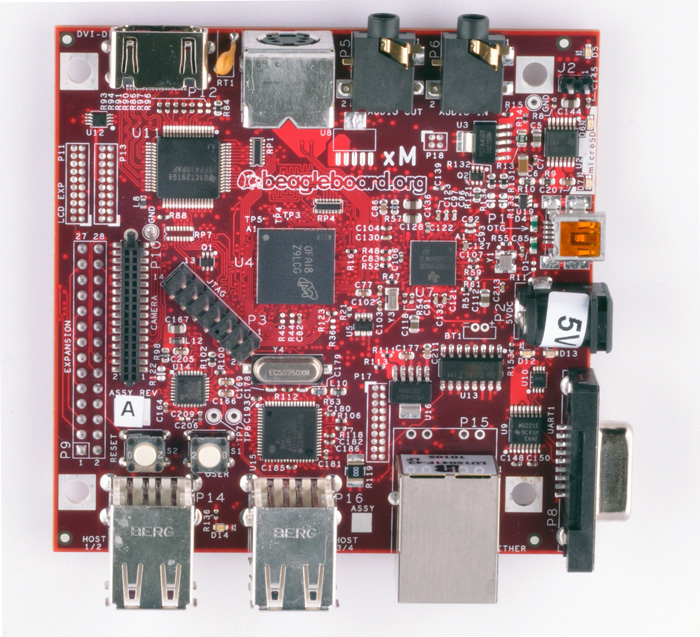
\includegraphics[scale=0.3]{intro_chapter/beagleboard_xm2.jpg} 
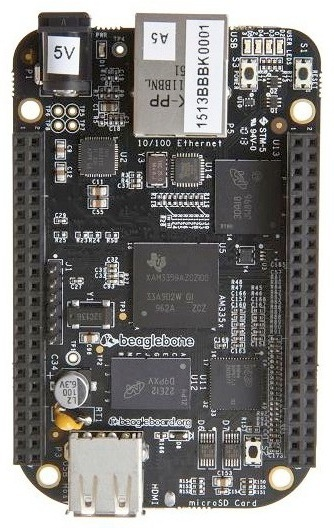
\includegraphics[scale=0.35]{intro_chapter/beagleboardblack.jpg} 
\caption{The BeagleBoard-xM (left) and BeagleBone Black (right) hardware platforms.}
\end{figure}

BeagleSNES originally began as a course project for a graduate embedded systems design class.  While the scope of the project was to port the SNES9X emulator to the BB-xM and then tune the board's Linux kernel for performance, things got a little out of hand.  The project kept growing in complexity and scope.  Over the span of four months, it matured into the initial release of the project that you see today.  The bootloader, Linux kernel, file system, and emulator of BeagleSNES have all been customized for functionality, stability, and performance.  These components were further customized when the project was ported to the BBB.

The source code for BeagleSNES, as well as the latest instructions for building, installing, and using the software, are freely available from \texttt{www.beaglesnes.org}.  Almost all of BeagleSNES is licensed under the GNU Public License (version 3) as open source software (OSS), but the emulator itself is licensed under a custom, non-commercial license.  What does this mean?  It means that you are welcome to examine the code, modify it, learn from it, and even use it in projects of your own.  But, you may not sell the system if it contains the emulator. 

The hardware of the SNES (CPU, GPU, memory, audio chipset, etc.) is quite different from the hardware of the BB-xM and BBB.  SNES software will never execute natively on these platforms, so BeagleSNES must \emph{emulate} the hardware of the SNES in software.  The inputs, outputs, and internal state of each piece of SNES hardware is represented as high-level source code (C and C++ code, in the case of BeagleSNES).  The 16-bit microprocessor of the SNES (the WDC 65C816) runs at a clock speed of 3.58 MHz.  This is much slower than the 32-bit ARM CPUs of the BB-xM (AM37x 800 MHz Cortex-A8) and BBB (AM335x 1 GHz Cortex-A8), meaning that there are enough resources available to dynamically translate every SNES program instruction, at the time that it would be executed on the SNES, into one or more ARM instructions and then execute them.  This \emph{just-in-time dynamic translation} approach has considerable overhead, but it is very effective in situations where the emulated system is much slower than the system performing the emulation.

\begin{figure}[h]
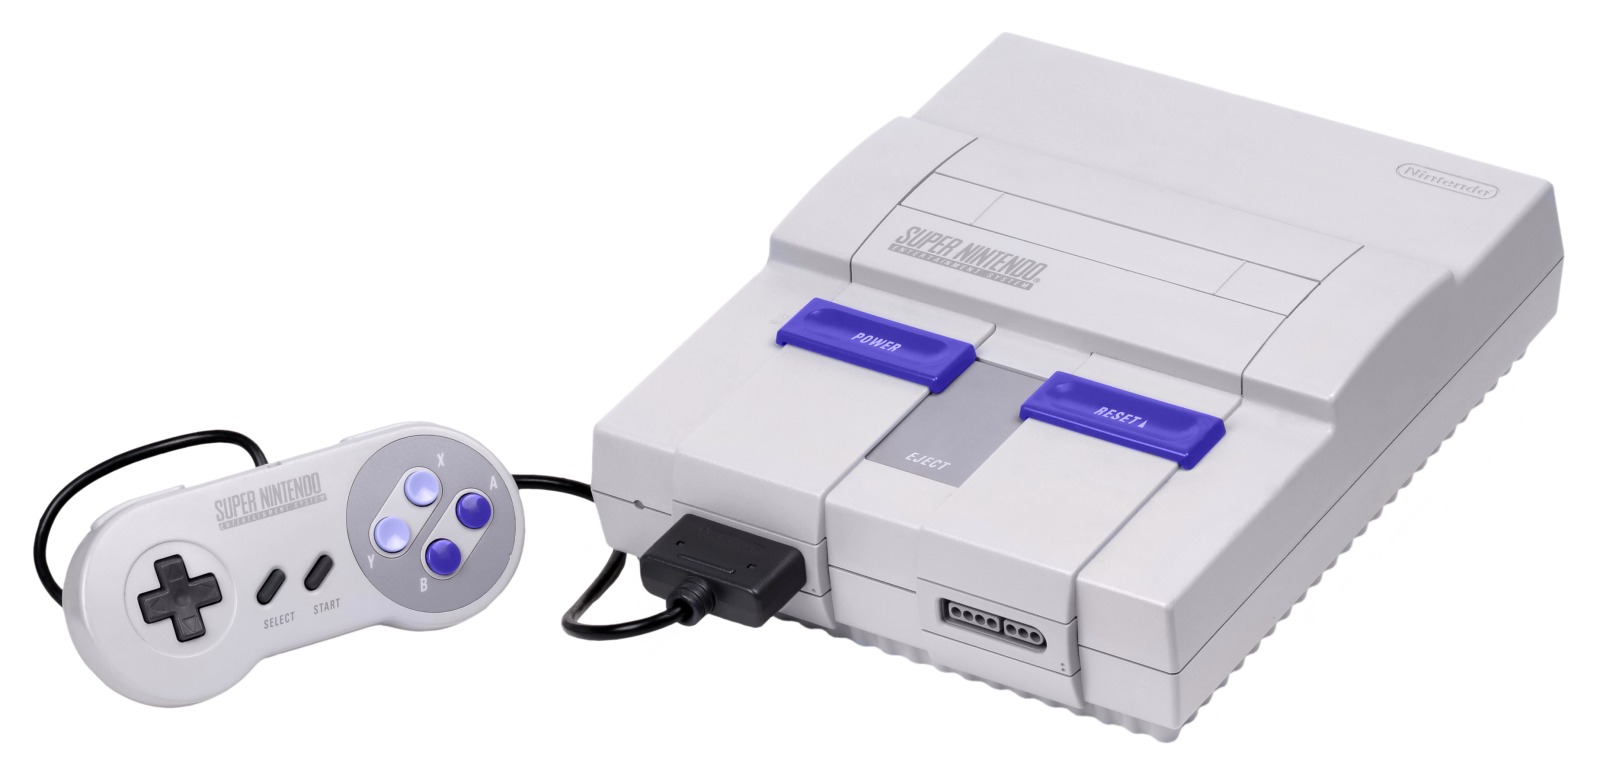
\includegraphics[scale=0.25]{intro_chapter/Super_Nintendo_North_America_Model.png}
\caption{The Super Nintendo Entertainment System\textregistered video game console.}
\end{figure}

Several SNES emulators currently exist, and BeagleSNES leverages this existing work (rather than "reinventing the wheel").  The SNES9X emulator\footnote{www.snes9x.com} was selected to serve as the emulator base for the project for the following reasons:

\begin{itemize}
\item All source code for the emulator is available, and all optimizations and additions made to it as part of BeagleSNES can be freely released as long as the terms of the SNES9X license are followed.
\item The source code for the emulator is cross-platform, meaning that its implementation is not tied to a particular display library or CPU architecture.
\item Its emulation compatibility is quite good, allowing it to run many different pieces of SNES software accurately.
\end{itemize}

While many architecture-specific performance optimizations exist in SNES9X (such as using x86-based assembly cores to accelerate the emulation), many of these improvements can't be used with the ARM-based BB-xM and BBB.  This limits the overall emulation speed of BeagleSNES, but the performance is generally acceptable.  

\section{Using This Manual}\index{Using This Manual}

This guide was written to help you to install and configure BeagleSNES.  It also contains technical information that provides details of how the system works and describes how to build the various components of the system from source.  Hopefully, this information will not only allow you to enjoy BeagleSNES for your own entertainment, but also allow you to use this work as a basis for whatever BeagleBoard-based system you might want to create.  

For any important aspects of the system that warrant additional attention, this manual uses the following box to highlight them:

\begin{updateWarn}
Be sure to pay attention to these boxes as you read through the manual.  They will alert you to any important or useful information that you should be aware of.
\end{updateWarn}

For any commands executed on the command line, this manual uses the following box:

\begin{commandBox}
\texttt{username@host\$  sudo ./execute\_this\_command}
\end{commandBox}

Each section of the guide contains information on a different aspect of BeagleSNES.  Section 1 is the introduction that you are reading right now.  Section 2 describes how to download and install the pre-made file system image of BeagleSNES.  For most end-users, this section will be the most important one to review.  Section 3 provides instructions on how to add ROMs to the BeagleSNES system and configure the game selection GUI and gamepad button mapping.  Section 4 is a troubleshooting guide to help you work through some of the common issues that people come across.  Section 5 gives step-by-step instructions on how to build the various pieces of the BeagleSNES system.  Section 6 provides more details about the configuration of the bootloader and Linux kernel used in BeagleSNES.  Section 7 describes several details of the audio, video, and input subsystems of BeagleSNES.  This will be of interest to developers that wish to review the technical details of how BeagleSNES interfaces with the BeagleBoard hardware.  Section 8 describes how BeagleSNES might be made into a portable system and discusses the LCD3 video target and GPIO input.  Section 9 acknowledges the people and projects that have contributed to the software and hardware that BeagleSNES is made from.  Finally, section 10 serves as a changelog of the project from release to release.

Enjoy using BeagleSNES!  Hopefully, you will learn a few things about embedded system design in the process, too!

\section{BeagleSNES License}\index{BeagleSNES License}

The bootloader, Linux kernel, and GNU utilities that make up the BeagleSNES system are all licensed under the GPL.  These components can be freely modified, shared, and even sold, as long as the terms of the GPL are followed.  Feel free to use them as a base for your own projects!

The license information for the BeagleSNES emulator application can be seen in figure 1.3.  This license is a slightly modified version of the SNES9X license, which directs you to the stock SNES9X license for all of the details.  It allows you to look at, learn from, and use BeagleSNES for personal use, but not to exploit it for commercial gain.  This is NOT GPL licensed software, but it is freeware.

\begin{figure}[h]
\lstinputlisting{license.txt}
\caption{The \texttt{beaglesnes-license.txt} file included in the BeagleSNES source code.}
\end{figure}

%----------------------------------------------------------------------------------------
%	INSTALLING CHAPTER
%----------------------------------------------------------------------------------------

\chapter{Installing BeagleSNES}

\section{Overview}\index{Overview}

BeagleSNES is more than just a single application.  It is a complete POSIX operating system environment, complete with a custom Linux kernel, a full file system, and configuration files that tell BeagleSNES how to behave for the end user.  Because of the general complexity of such a large system, it can sometimes be difficult to get everything up and running smoothly.  This section will tell you how to download and install BeagleSNES so that you can get started using it as quickly and painlessly as possible.  

\begin{figure}[h]
\centering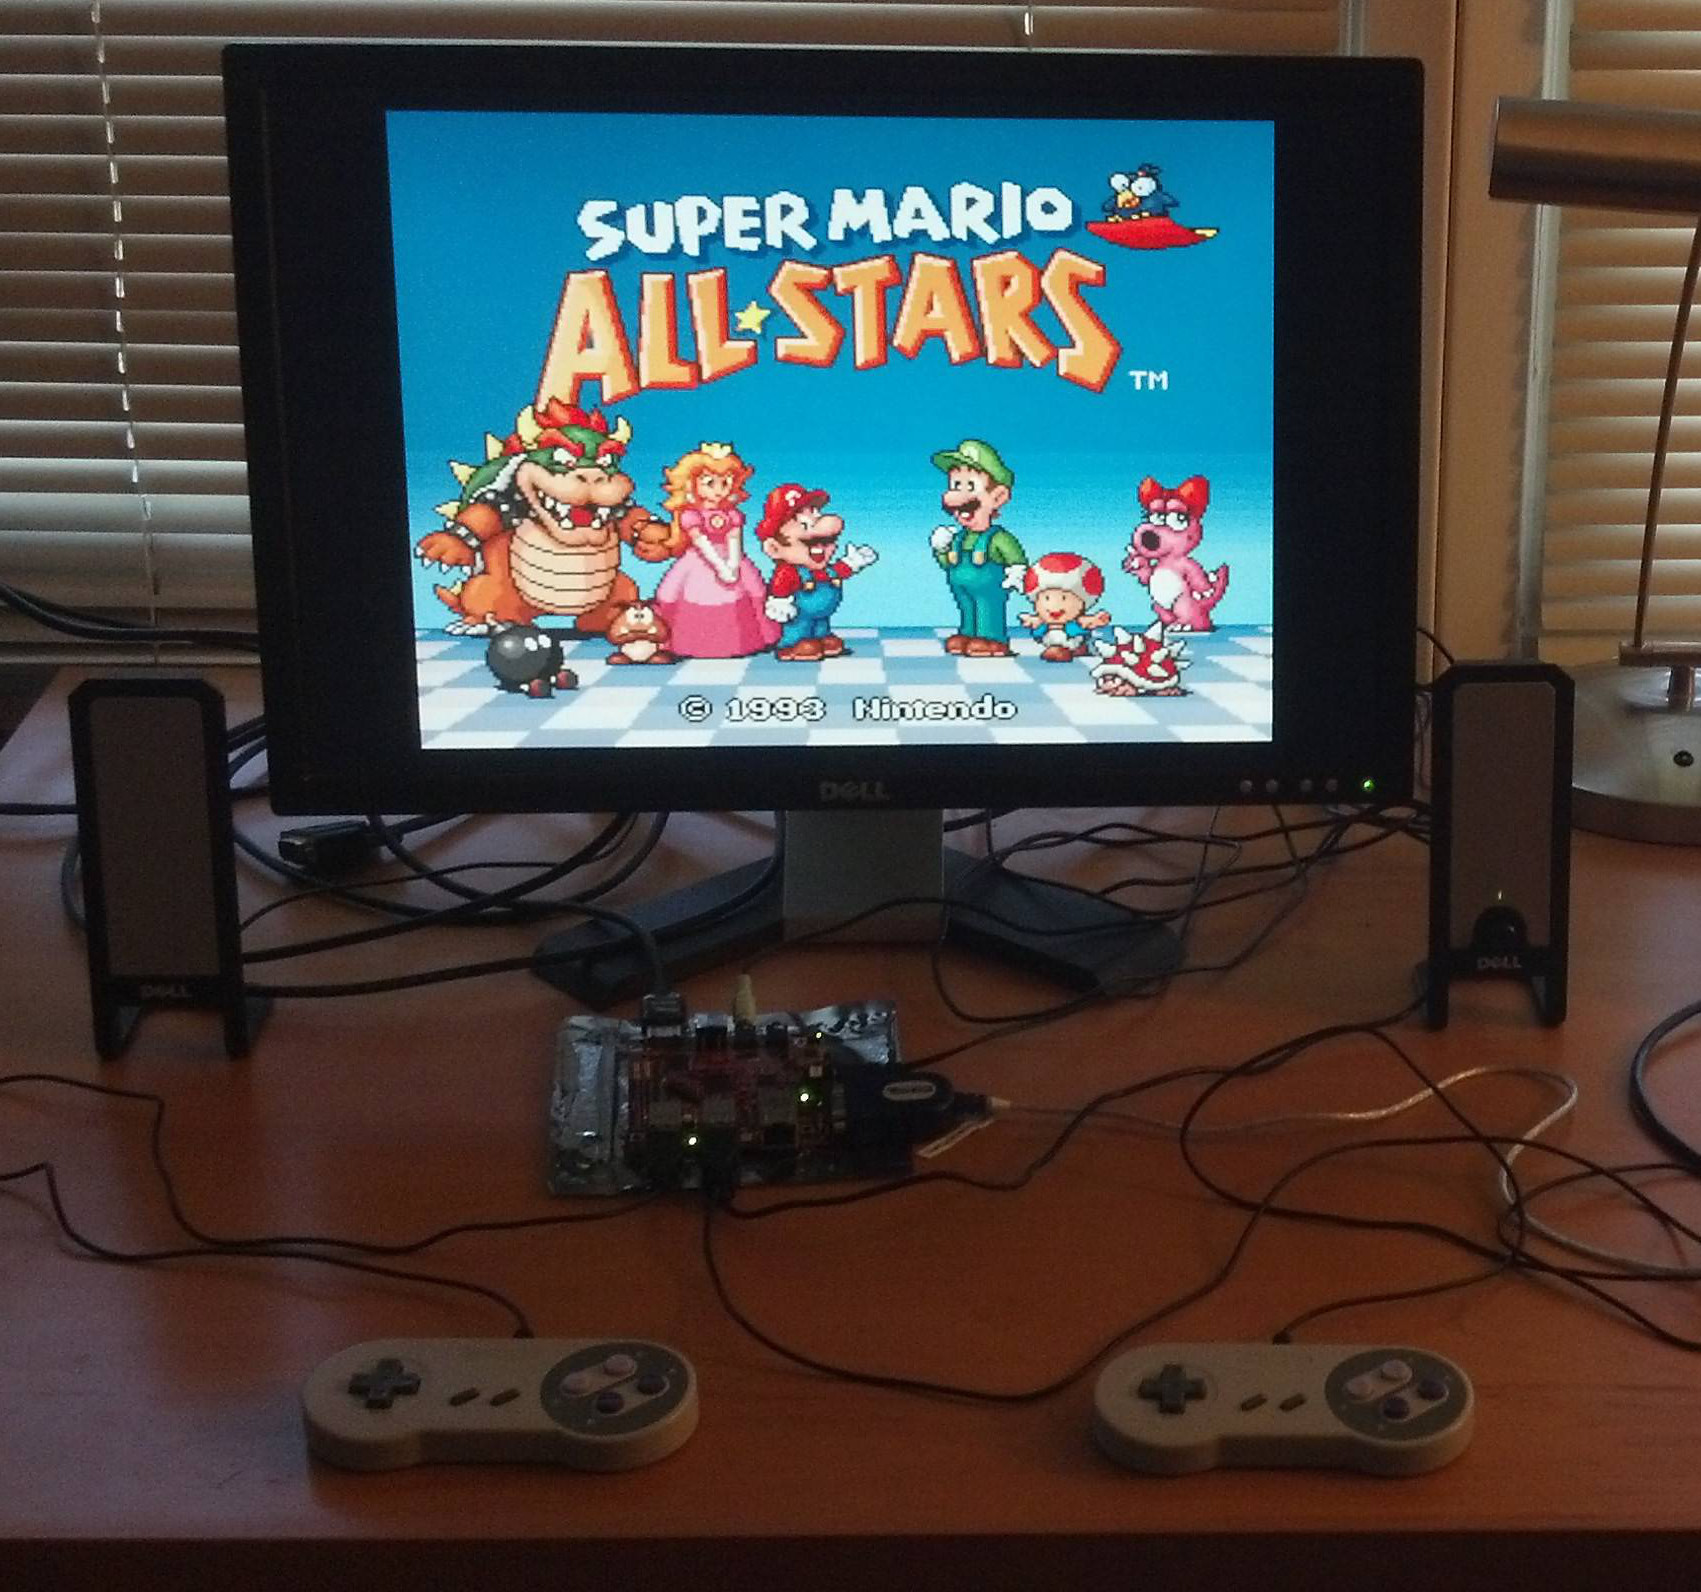
\includegraphics[scale=0.10,clip=true,trim=0 40 0 0]{install_chapter/BBxM_version.jpg}
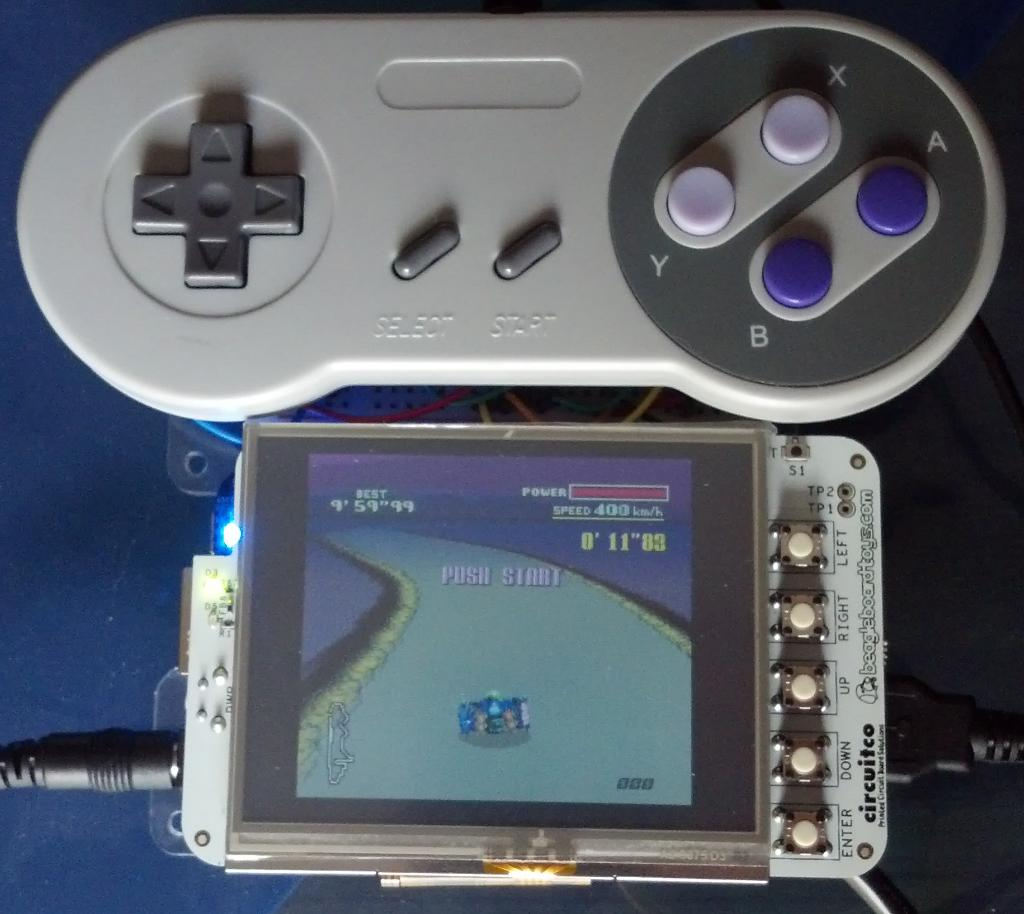
\includegraphics[scale=0.17]{install_chapter/LCD3_version.jpg}
\caption{The 0.5 release of BeagleSNES, running on the BB-xM with DVI digital video output (left) and on the BBB with the LCD3 cape (right).}
\end{figure}

All source code for the project, as well as a full file system image of a complete BeagleSNES system, have been made available for download.  Most users will only wish to try out BeagleSNES, rather than hack on its source code, so this section will focus on using the full file system image.  Prior to starting, you'll need the following items:

\begin{itemize}
\item Either a BB-xM hardware platform that is at least revision C or a BBB platform that is at least revision A5A.  Earlier revisions have not been tested and are not suggested.
\item An external power supply to provide full power to the system.  Powering via USB will not provide the necessary amount of current.
\item An HDMI-to-DVI cable (BB-xM) or microHDMI-to-HDMI cable (BBB), and a television or monitor capable of displaying the digital video signal.  Or, if you may wish to instead use a Circuitco LCD3 cape board for displaying video for the BBB.
\item For the BB-xM, external speakers or a headset for listening to the audio output\footnote{Even when using an HDMI-to-HDMI cable for the video, audio will not be transmitted over the cable.  This is because the signal being transmitted over the HDMI cable is actually a DVI signal (video only), rather than an HDMI signal that contains both video and audio data.}.  The audio for the BBB is sent over the HDMI connection. 
\item A microSD card with a capacity of at least 4 GB.  BeagleSNES will rewrite the partition table on this card, so make sure that it does not contain any data that you need.
\item Copies of the software ROMs that you wish to use with BeagleSNES.
\item One or two Tomee\texttrademark USB SNES Gamepad controller(s)\footnote{Several online vendors offer this particular USB controller for sale. It is the only controller that will be officially supported for BeagleSNES.}. The BB-xM supports using one or two controllers, but the BBB only supports one unless you use an external USB hub to provide additional USB ports.  \emph{USB controllers other than the Tomee\texttrademark will work with BeagleSNES}, but they will most likely need their buttons remapped.
\end{itemize}

\begin{updateWarn}
While many SNES ROMs are widely available on the web, possession of these ROMs is generally considered to be piracy of commercial software. No ROMs are provided in the BeagleSNES file system images, and no help in obtaining ROMs will be given.  You're on your own.
\end{updateWarn}

\section{Downloading}\index{Downloading}

There are two BeagleSNES file system images available for download. The first is a microSD card image that contains a complete BeagleSNES system (bootloader, kernel, file system, etc.).  The second is a tarball of only the directory structure that includes the BeagleSNES application, its associated resources, and sample configuration files.  This image is intended for more advanced users that wish to add the BeagleSNES emulator into an existing file system environment that they have created.  The complete microSD card image will be referred to as the \emph{full system image}, and the tarball of the BeagleSNES directory structure will be referred to as the \emph{application image}.  The contents of the application image already exist inside of the full system image.

Direct download links to the latest versions of all BeagleSNES software components are available at \texttt{www.beaglesnes.org}.  SourceForge hosts all of the files for BeagleSNES\footnote{\texttt{https://sourceforge.net/projects/beaglesnes/files/}}, but \texttt{www.beaglesnes.org} should first be consulted for any additional information that you might need about the latest version of BeagleSNES prior to downloading. 

\section{Installing}\index{Installing}

The easiest way to install BeagleSNES is to write the full system image to a microSD card and then boot your BBB or BB-xM from that card. The speed class of the card is not all that important, but all of the BeagleSNES development was performed using a class 10 card. Slower speed classes may increase the time needed for a system boot, but otherwise the impact on the performance of BeagleSNES is assumed to be negligible.

Some advanced BeagleBoard users may already have a working file system, kernel, etc. on their system and only wish to install the BeagleSNES application. For those people, the application image can be copied into their existing file system. Libraries used by BeagleSNES (SDL, SDL\_mixer, etc.)\footnote{A full list of the libraries used can be seen in section 3.4.} are not shipped with the application image because you might not have built your particular kernel with the same features that are in the BeagleSNES kernel (ALSA, framebuffer console, etc.). It will be up to you to install the needed libraries on your system in a fashion that is compatible with your current kernel features. 

In addition, BeagleSNES needs to be started at boot. There is a script named \emph{service.sh}\footnote{This script not only launches the emulator, but it also uses \texttt{nice} to adjust the priority of the emulator by -20. This effectively makes the emulator the highest-priority user space process running on the system.} in the application image that should be called by a boot \texttt{cron} job, the \texttt{rc.local} script, or other similar mechanism upon system start-up. Modify the path to the BeagleSNES directory in \emph{service.sh} to point to the path where you have installed the application image on your system.

To copy the full system image to your microSD card, first download the image and then use \texttt{bunzip2} to decompress it.  Execute a Unix \texttt{dd} command similar to the following to write the image to your microSD card\footnote{Windows users can use the Win32 Disk Imager utility to write the image to the microSD card.  Download it at: \texttt{http://sourceforge.net/projects/win32diskimager}}:

\begin{commandBox}
\texttt{username@host\$ sudo dd if=beaglesnes\_system.img of=/dev/sdX bs=1M}
\end{commandBox}

This command will take a little while to run, so be patient. The output file parameter (\texttt{of}) will may vary depending upon what device represents the microSD card on your particular Linux system. For most systems, \texttt{/dev/sdX} (\texttt{sda}, \texttt{sdb}, etc.) will represent the microSD card. On others, you might see \texttt{/dev/mmcblkX} instead, where the "X" is a number (0 for the first microSD card, 1 for the second, etc.). It is up to you to determine which it is. Don't guess and try different parameters without knowing for sure! A bad guess might end up with your accidentally overwriting data on some other device in your system!

Once the full system image is copied onto the microSD card, the card will contain two file system partitions.  The first partition is the \texttt{VFAT} \texttt{/boot} partition.  The kernel and bootloader live in this partition, as do the BeagleSNES configuration files and any ROMs and game images that you've copied to the system.  The second partition is the \texttt{EXT4} \texttt{/rootfs} partition where the BeagleSNES application and base Linux distribution live.  The \texttt{VFAT} filesystem on the \texttt{/boot} partition is understood by Windows, the various OSes of Apple hardware, and Unix OSes like Linux and FreeBSD, so it is simple to add new games and change configuration settings no matter which OS you use to do so.  

Insert the microSD card with the BeagleSNES image into your board and then power the board up.  After about 10-12 seconds, the game selection menu will appear, begin playing background music, and display with the default dummy game entries. 

\begin{updateWarn}
When using BeagleSNES on a BBB, you do \emph{not} have to hold down the "user boot" button during boot.  The BeagleSNES \texttt{uEnv.txt} file is written such that the bootloader on the BBB's eMMC understands that it should boot from the microSD card and it will do so automatically.
\end{updateWarn}

\begin{updateWarn}
A freshly-downloaded BeagleSNES microSD card image has a default boot configuration for a BBB using HDMI for audio and video.  It \emph{will not boot} for other configurations (BBB with LCD3 or BB-xM) until you change the bootloader and \texttt{uEnv.txt} files. The next section explains how to change the default bootloader and \texttt{uEnv.txt} files over to their respective versions for booting BeagleSNES on the BBB with LCD3 or the BB-xM.
\end{updateWarn}


%----------------------------------------------------------------------------------------
%	CONFIGURING CHAPTER
%----------------------------------------------------------------------------------------

\chapter{Configuring and Using BeagleSNES}

\section{Overview}

Within the full system image, the BeagleSNES application lives in the \emph{application root directory}: \texttt{/home/ubuntu/beaglesnes}. To make things easier for the end-user, all of the standard configuration files that control game configuration, controller button mapping, etc. are located inside of the \texttt{/boot} partition.  The \texttt{/boot} partition uses a \texttt{VFAT} filesystem, so files can be easily copied to it or modified by mounting the microSD card on a Windows, Mac, or Linux system and making the desired changes.  

\begin{updateWarn}
When logging into a running BeagleSNES system, use the username "ubuntu" and password "temppwd". You can use the "ubuntu" account to \texttt{sudo} any administrative commands that you feel need to be performed on the system.
\end{updateWarn}

\section{Choosing a Boot Configuration}\index{Choosing a Boot Configuration}

BeagleSNES supports three boot configurations:
\begin{itemize}
\item The BB-xM using DVI for video and the BB-xM audio jack for audio via external speakers.
\item The BBB using HDMI for audio and video.
\item The BBB using an LCD3 cape for video and some other hardware (such as a USB audio device) for audio.
\end{itemize}
The default configuration for the full system image is for the BBB using HDMI.  While the BBB and BB-xM kernels have different names and can exist side-by-side in the \texttt{/boot} partition, the bootloader and \texttt{uEnv.txt} files for each platform have the same names and can't co-exist in the same location.  To address this issue, three scripts have been added to the \texttt{/boot} partition to change the current boot configuration to one of the other configurations.  The \texttt{setup\_BBB\_HDMI.sh} script makes the BBB with HDMI the active boot configuration by copying the bootloader and \texttt{uEnv.txt} files from the \texttt{BBB\_HDMI} subdirectory into the root of the \texttt{/boot} partition.  The \texttt{setup\_BBB\_LCD3.sh} script makes the BBB with LCD3 the active boot configuration in the same manner (copying files from the \texttt{BBB\_LCD3} subdirectory).  The \texttt{setup\_BBxM.sh} script will do the same, but it will copy the files from the \texttt{BBxM} subdirectory and make those BBxM files the active ones for the system.  You won't be able to execute these scripts while the system is running (i.e. a BBB-configured full system image won't even boot on a BB-xM, so you will not be able to shell into the system to run \texttt{setup\_BBxM.sh}), so you must mount the \texttt{/boot} partition of the microSD card on a Linux system, \texttt{cd} into the partition, and then execute the script by using one of the following commands:

To set the system to BB-xM: 

\begin{commandBox}
\texttt{username@host\$  sudo sh ./setup\_BBxM.sh}
\end{commandBox}

To set the system to BBB with HDMI: 

\begin{commandBox}
\texttt{username@host\$  sudo sh ./setup\_BBB\_HDMI.sh}
\end{commandBox}

To set the system to BBB with LCD3: 

\begin{commandBox}
\texttt{username@host\$  sudo sh ./setup\_BBB\_LCD3.sh}
\end{commandBox}

\begin{updateWarn}
Alternatively, you can simply copy the files from the desired boot configuration subdirectory (\texttt{BBxM}, \texttt{BBB\_HDMI}, \texttt{BBB\_LCD3}) into the root of the \texttt{/boot} partition to replace the existing boot files.  This is the easiest approach for Windows users that are unable to execute the shell scripts.
\end{updateWarn}

All three \texttt{uEnv.txt} files have two different configuration settings within the \texttt{uEnv.txt} file itself: the "fast boot" configuration and the "development boot" configuration.  By default, all of the \texttt{uEnv.txt} files are set up for fast boot.  The differences between the fast and development boot configurations are the boot time and which OS features are enabled.  Fast boot uses BeagleSNES as the \texttt{init} process of the Linux system.  Only the bare minimum of system daemons are started, and only the file systems required for BeagleSNES operation are mounted.  Networking is not enabled under this configuration, and you also won't be able to build the BeagleSNES in-place on the hardware.  But, the boot time for the system is only about 10-12 seconds.  The development boot configuration uses the standard Linux \texttt{init} daemon as the \texttt{init} process, and it enables all features of the system, but it requires a boot time of about 20 seconds.  Instructions on how to switch between the fast boot and development configurations are given in Section 6.  Unless you are planning on doing BeagleSNES development, using the microSD card image for your own development project, or need network access to transfer ROMs to your microSD card, stick with using the fast boot configuration. 

\section{Configuring BeagleSNES}\index{Configuring BeagleSNES}

Once the image has been copied onto the microSD card and configured for your platform, you have two options for configuring the BeagleSNES application and loading game ROMs into it. The first method is to mount the microSD card on another system and then access the \texttt{/boot} partition directly to copy and modify files. This is by far the easier method, since you are free to copy files back and forth between your system and the BeagleSNES file system quickly and easily. 

The second method is to insert the microSD card into your BB-xM or BBB, power up the system, and then use the ethernet interface\footnote{For the BBB, you can also use an FTDI cable to shell into the system to make configuration changes (though you won't be able to copy files).  The FTDI interface will work for both fast boot and networking configurations.} to shell into your BeagleSNES system and access the file system remotely. The full system image uses DHCP to request an IP address when an ethernet cable is attached to the system. You can use utilities like \texttt{scp} to copy files to and from the system and \texttt{ssh} to shell into the system and edit files locally. You will have to manually determine what IP has been assigned to the device by performing a broadcast ping or by looking at the administration interface of your router or DHCP server to see which IPs are in use. Your BeagleSNES system will show up in the administration interface with the hostname \texttt{beaglesnes}. 

\begin{updateWarn}
If you are using a fast boot configuration, networking will not be enabled and this method can't be used.
\end{updateWarn}

There are three things that must be completed before your BeagleSNES is usable:

\begin{itemize}
\item Descriptions and information for each game listed in the selection menu must be added to the \texttt{games.xml} file. 
\item ROM and image files associated with each game listed in the selection menu must be copied into the file system.
\item Gamepads and GPIO inputs must be configured to use the proper button mapping in the \texttt{games.xml} file if the default mapping isn't correct.
\end{itemize}

Adding game information is covered in Section~\ref{sec:games_xml}.  Copying ROMs and images into the file system is covered in Section~\ref{sec:add_files}.  Configuring button mappings for gamepads is covered in Section~\ref{sec:conf_gamepad}.

For the current release, BeagleSNES's game selection menu supports having a large, but not unlimited, number of game titles. At least one game must exist in the actual system, of course, but there is no specified upper limit.  As more games are added to the menu, more system RAM will be consumed and the start-up time for the BeagleSNES application will increase.  While no stress tests have been performed to see just how many games can be added to the system, it should easily handle several hundred games.

All configuration and data files for BeagleSNES are located in the \texttt{beaglesnes} subdirectory in the root directory of the \texttt{/boot} partition.  On the running BeagleSNES system, the location of the \texttt{beaglesnes} directory is \texttt{/boot/uboot/beaglesnes}.  If the microSD card with BeagleSNES is mounted on a Windows system, the path to the \texttt{beaglesnes} directory is off the root of the drive that the \texttt{/boot} partition is mounted as.  For example, if the microSD card is inserted into a Windows system and the \texttt{/boot} partition becomes drive \texttt{E:}, the path of the \texttt{beaglesnes} directory is \texttt{E:\textbackslash beaglesnes}.

\subsection{Modifying games.xml}\index{Configuring BeagleSNES}\label{sec:games_xml}

The \texttt{games.xml} should be the only configuration file that you will need to modify for BeagleSNES.  It is an XML file that describes the button mapping for your controllers, GPIO mapping for controls, and the game descriptions, box images, and ROM files associated with each game listed in the game selection menu. \texttt{games.xml} is located in the \texttt{beaglesnes} subdirectory of the \texttt{/boot} partition.

\begin{table}[h]
\centering
\begin{tabular}{| l | l | l | l |} \hline
%\toprule
\textbf{XML Tag} & \textbf{Purpose} & \textbf{Minimum} & \textbf{Maximum}\\ \hline
%\midrule
<config> & Top level tag of XML file & 1 & 1 \\ \hline
<gpio> & Mark section of GPIO buttons & 0 & 1 \\ \hline
<gpio\_*> & Specific GPIO button mapping & 0 & 1 per <gpio> \\ \hline
<player1/2> & Mark section of button mapping & 0 & 2 \\ \hline
Various tags & Map buttons (<vaxis>, <select>, etc.) & 0 & 1 per <player?> \\ \hline
<pause\_combo> & Combo that triggers pause menu & 0 & 1 \\ \hline
<pause\_key> & Button that is part of the pause combo & 0 & No limit \\ \hline 
<snes> & Mark section of all SNES games & 1 & 1 \\ \hline
<game> & Mark section of a single game & 1 & No limit \\ \hline
<title> & Title of a game & 1 per <game> & 1 per <game> \\ \hline
<rom> & Filename of a game ROM & 1 per <game> & 1 per <game> \\ \hline
<image> & Filename of a game image & 0 & 1 per <game> \\ \hline
<genre> & Genre of a game & 0 & 2 per <game> \\ \hline
<year> & Year of a game & 0 & 1 per <game> \\ \hline
<text> & Description of a game & 0 & 5 per <game> \\ \hline
%\bottomrule
\end{tabular}
\vspace{-0.1in}
\caption{XML tags of the BeagleSNES \texttt{games.xml} file.}\label{tbl:games_xml}
\end{table}

The XML tags used in the \texttt{games.xml} file are described in Table~\ref{tbl:games_xml}. A sample \texttt{games.xml} that demonstrates some of these tags is shown in Figure~\ref{fig:games_xml}.  Two sample game entries are listed.  The first game, \texttt{GameTitle1}, has an entry that defines every possible field.  The second game, \texttt{GameTitle2}, has an entry that defines only the bare minimum fields required to make a valid entry (\texttt{<title>} and \texttt{<rom>}).  If the other tags are not defined, default values are used in their place. A full sample \texttt{games.xml} file is included in both the full and application file system images. It contains a dummy configuration for a menu with 10 ROMs, gamepad button mappings for the player 1/2 controllers, GPIO inputs, and a pause menu button combo.  The sample will act as a template to help guide you as you configure BeagleSNES for your own use.

\begin{figure}[h]
\begin{verbatim}<?xml version="1.0"?>
<config>
<snes>
  <game>
    <title>GameTitle1</title>
    <rom>filename1.smc</rom>
    <image>box_image1.png</image>
    <year>1999</year>
    <genre>Genre1</genre>
    <genre>Genre2</genre>
    <text>Description text line 1</text>
    <text>Description text line 2</text>
    <text>Description text line 3</text>
    <text>Description text line 4</text>
    <text>Description text line 5</text>
  </game>
  <game>
    <title>GameTitle2</title>
    <rom>filename2.smc</rom>
  </game>
  ... More <game></game> tags go here for more games ...
</snes>
</config>\end{verbatim}
\vspace{-0.3in}
\caption{Example of a \texttt{games.xml} file.}\label{fig:games_xml}
\end{figure}

\begin{updateWarn}
There is no need to add path prefixes, such as \texttt{image/} or \texttt{rom/}, when specifying the ROM or box image filenames in \texttt{games.xml}. BeagleSNES already knows which directories to look in to find those files, so only the name of the file itself needs to be specified.
\end{updateWarn}

\begin{updateWarn}
There are five special characters (`` \texttt{``} '', ``\texttt{\&}'', ``\texttt{`}'', ``\texttt{<}'', ``\texttt{>}'') that have a special meaning in XML, so you must replace each one with a special \emph{predefined entity} in the XML file. Each predefined entity is a placeholder that will be replaced with the appropriate character when the text is actually rendered on the screen.  The predefined entities for `` \texttt{``} '', ``\texttt{\&}'', ``\texttt{`}'', ``\texttt{<}'', and ``\texttt{>}'' are ``\texttt{\&quot;}'', ``\texttt{\&amp;}'', ``\texttt{\&apos;}'', ``\texttt{\&lt;}'', and ``\texttt{\&gt;}'', respectively. For example, the title ``\texttt{Pocky \& Rocky}'' would be entered as ``\texttt{Pocky \&amp; Rocky}'' in the XML file.
\end{updateWarn}

\subsection{Adding ROMs and Images}\index{Configuring BeagleSNES}\label{sec:add_files}

Each SNES ROM must be copied into the \texttt{rom} subdirectory of the \texttt{beaglesnes} directory of the \texttt{/boot} partition.  The downloadable image files for BeagleSNES do not include any SNES ROMs, so the system will not do anything useful until you add your own ROMs to the file system.  The SNES ROMs used with BeagleSNES must be NTSC SNES titles. ROMs can be compressed (\texttt{.zip} or \texttt{.gz} file extension) or uncompressed (\texttt{.smc} file extension).  If a particular title is able to run on the SNES9X emulator, then it will most likely run on BeagleSNES.  Add as many SNES ROMs as you like into the \texttt{rom} directory, but only ROMs specified in the \texttt{games.xml} file will appear in the game selection menu.

Each box or screenshot image must be copied into the \texttt{image} subdirectory of the \texttt{beaglesnes} directory of the \texttt{/boot} partition. The game selection menu is designed to accommodate a 200x145 pixel PNG image for the box image. This image size has the same aspect ratio as the original SNES cartridge box.  Some SNES titles (such as Japanese releases that were never released in the North American market) originally came in a box with a different aspect ratio. As long as the height of the image does not exceed 145 pixels, the extra width of the image should still fit in the menu screen without a problem.

\begin{figure}[h]
\centering
\includegraphics[scale=3.0]{install_chapter/blank_box.png}
\caption{The included 200x145 pixel \texttt{blank\_box.png} placeholder image that is used if no image is specified.}
\end{figure}

\subsection{Configuring Gamepad Button Mapping}\index{Configuring BeagleSNES}\label{sec:conf_gamepad}

There are a variety of USB human interface devices (HIDs) that are recognized as joysticks by the Linux kernel's USB subsystem.  Not all of these devices are true joysticks (they might be gamepads, or even devices that looks nothing like a game controller), but they all fall within the same category of "close enough in functionality to a joystick to be treated as such by the kernel".  While  these joysticks and gamepads can be used to provide input to BeagleSNES, the physical buttons of each controller must first be mapped to the "logical" buttons inside BeagleSNES that correspond to the buttons of the original SNES controller.  

\begin{figure}[h]
\centering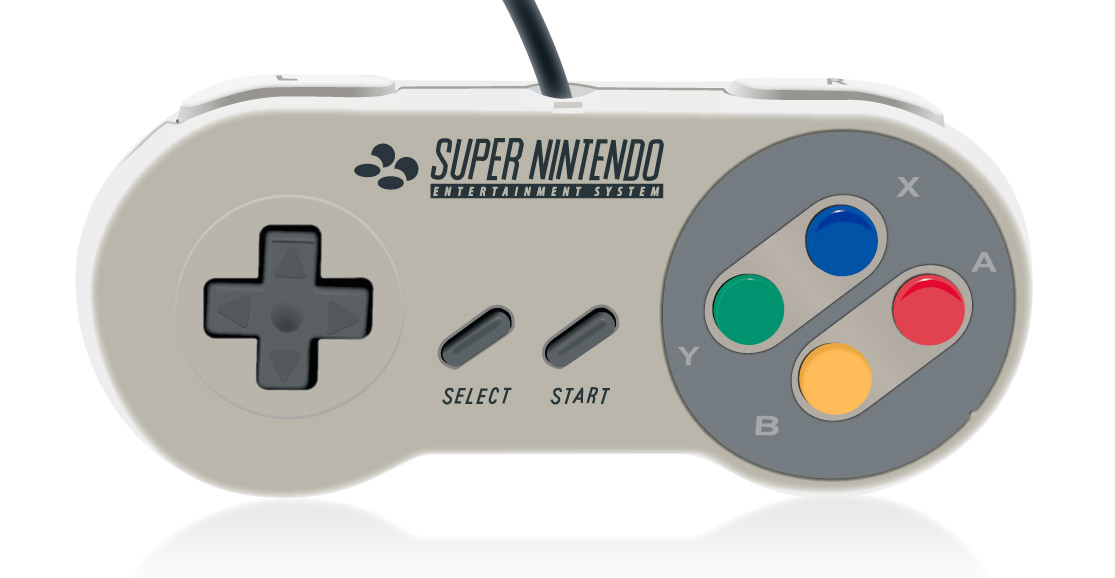
\includegraphics[scale=0.25,clip=true,trim=75 80 75 60]{config_chapter/snes_controller.jpg}
\caption{The original SNES controller. The L (left) and R (right) shoulder buttons are located on the top edge of the controller.}\label{fig:snes_controller}
\end{figure}

As a reference, the original SNES controller is shown in Figure~\ref{fig:snes_controller}.  This controller has a directional pad that provides two "axes" for directional input (an up/down axis and a left-right axis).  It also provides a total of eight buttons: the rectangular start and select buttons, four round input buttons for A/B/X/Y, and two shoulder buttons on the edge of the controller for L (left) and R (right).

BeagleSNES uses the configuration file \texttt{snes9x.conf} to define the \emph{default} mappings between physical joystick buttons and axes to the logical buttons and axes used by the emulator.  \texttt{snes9x.conf} is located in the \texttt{beaglesnes} directory of the \texttt{/boot} partition.  The button mapping settings are located in a section within the \texttt{snes9x.conf} named \texttt{[BeagleSNES Controls]}.  Previous versions of BeagleSNES required users to change this section to map SNES gamepad buttons to the buttons of your joystick.  But, the \texttt{snes9x.conf} configuration file is now completely ''off-limits'' for the end-user.  All button mappings are now set using the \texttt{games.xml} file.

\begin{updateWarn}
Don't touch the \texttt{snes9x.conf} file!  All configuration settings are now made via the \texttt{games.xml} file.
\end{updateWarn}    

The \texttt{<player1>} and \texttt{<player2>} tags in the \texttt{games.xml} file describe button mappings between your joystick and the SNES gamepad. Figure~\ref{fig:controller_map} demonstrates the use of these tags.  The default button mappings are used for any controller or button not explicitly mentioned in the \texttt{games.xml}.  The only exception to this is the \texttt{<pause>} tag.  If you have a joystick with enough buttons to map all of the SNES controller buttons and still have at least one button to spare, the extra button can be mapped to trigger the pause menu.  Unless the \texttt{<pause>} is explicitly mapped, though, no default is mapped.  

\begin{figure}[h]
\begin{verbatim}<?xml version="1.0"?>
<config>
<player1>
  <vaxis>1</vaxis>
  <haxis>0</haxis>
  <L>4</L>
  <R>5</R>
  <A>1</A>
  <B>2</B>
  <X>0</X>
  <Y>3</Y>
  <select>8</select>
  <start>9</start>
  <pause>11</pause>
</player1>
<player 2>
  ... similar tags go here for the player 2 controller ...
</player2>
... other tags go here ...
</config>\end{verbatim}
\caption{Controller button mapping portion of the \texttt{games.xml} file.}\label{fig:controller_map}
\end{figure}

\subsection{Configuring A Pause Combination}\index{Configuring A Pause Combination}\label{sec:conf_pause}

If you can't spare an extra button to trigger the pause menu, you can map the pause to a combination of buttons. When this button combo is pressed on the player 1 controller, the pause menu will trigger.  For example, you can map the left and right trigger buttons and the start and select buttons together as a pause button combo.  When all four are pressed simultaneously, the pause menu triggers.  Because you don't want the pause button combo to be a set of buttons that will interfere with gameplay, selecting three to four buttons for the combo is advised. 

The pause combo is defined by using two tags: \texttt{<pause\_combo>} and \texttt{<pause\_key>}.  An example pause combo that uses the left and right trigger buttons and the start and select buttons is shown in Figure~\ref{fig:pause_combo}.

\begin{figure}[h]
\begin{verbatim}<pause_combo>
  <pause_key>4</pause_key>
  <pause_key>5</pause_key>
  <pause_key>8</pause_key>
  <pause_key>9</pause_key>
</pause_combo>\end{verbatim}
\caption{XML for a pause button combo in the \texttt{games.xml} file.}\label{fig:pause_combo}
\end{figure}

This particular pause combo assumes the same button mapping as seen in the \texttt{<player1>} tag in Figure~\ref{fig:controller_map}.  For example, the first \texttt{<pause\_key>} of the combo is for button \texttt{4}.  The \texttt{<player1>} tag maps \texttt{4} to the left trigger button in the \texttt{<L>} tag. If the button mapping changes in the \texttt{<player1>} tag, the \texttt{<pause\_key>} tags must be changed to match it. 

\subsection{Configuring GPIOs For Input}\index{Configuring GPIOs For Input}\label{sec:config_gpio}

The BBB platform has support for mapping GPIO inputs as player 1 controller inputs.  The SNES directional pad and buttons, and even the pause button, can be mapped to GPIOs.  A maximum of 13 GPIO inputs (four for the d-pad, eight for buttons, and one for pause) can be mapped using a contiguous block of the BBB's pins (P8.7 through P8.19). Mapping the GPIOs uses the \texttt{<gpio>} tag and a series of \texttt{<gpio\_*>} tags that specify particular SNES controller buttons and controls. Figure~\ref{fig:gpio_mapping} shows a sample GPIO mapping.

\begin{figure}[h]
\begin{verbatim}
<gpio>
  <gpio_gpleft>1</gpio_gpleft>
  <gpio_gpright>2</gpio_gpright>
  <gpio_gpup>3</gpio_gpup>
  <gpio_gpdown>4</gpio_gpdown>
  <gpio_L>5</gpio_L>
  <gpio_R>6</gpio_R>
  <gpio_A>7</gpio_A>
  <gpio_B>8</gpio_B>
  <gpio_X>9</gpio_X>
  <gpio_Y>10</gpio_Y>
  <gpio_select>11</gpio_select>
  <gpio_start>12</gpio_start>
  <gpio_pause>13</gpio_pause>
</gpio>\end{verbatim}
\caption{XML for mapping GPIOs to SNES controls in the \texttt{games.xml} file.}\label{fig:gpio_mapping}
\end{figure} 
 
Each individual \texttt{<gpio\_*>} tag contains a number from one through thirteen.  These numbers correspond to the pins on the P8 header of the BBB.  Pin P8.7 is 1, pin P8.8 is 2, etc. up through pin P8.19, which is 13.  If a particular pin number is not mapped, it won't be initialized by BeagleSNES.  For more information on the hardware details of trigger GPIOs for input to BeagleSNES, check out Section~\ref{sec:gpio_hardware}.

\section{Using BeagleSNES}\index{Using BeagleSNES}

Once the system has been configured, it is now ready for use. BeagleSNES expects either one or two USB gamepads to be plugged in.  Two host USB ports on the BB-xM system have been designated by BeagleSNES as the gamepad ports: one for "player one" and the other for "player two".  \emph{Any gamepad that is not plugged into one of these designated USB ports is ignored.} Figure~\ref{fig:bbxm_usb} shows which two BB-xM USB ports are designated for the gamepads. 

\begin{figure}[h]
\centering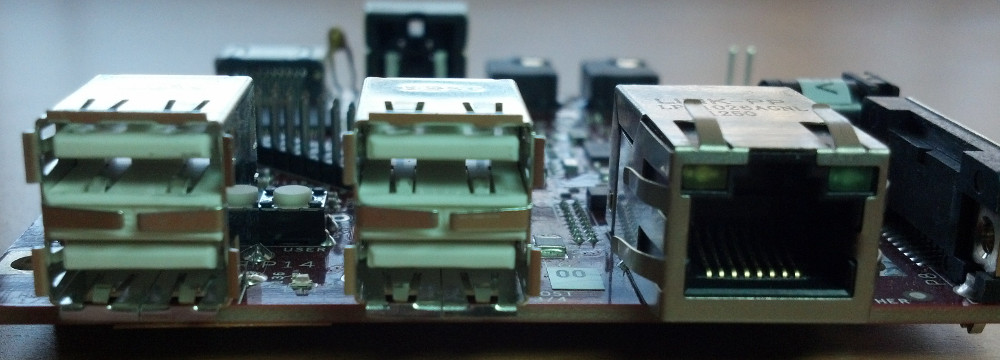
\includegraphics[scale=0.4]{install_chapter/usb_ports.jpg}
\caption{The USB ports of the BB-xM.  The top-left USB port is reserved for the "player one" gamepad, and the top-right USB port is reserved for the "player two" gamepad.}\label{fig:bbxm_usb}
\end{figure}

The BBB has only one host USB port, so there are two options for using gamepads with the system.  The first option is to plug a gamepad into the host USB port.  This is the port for the "player one" gamepad, and no "player two" gamepad can be used.  The second option is to plug a USB hub into the host USB port and then plug one or two gamepads into the hub.  Much like the host USB ports of the BB-xM, one port of the hub will be the "player one" port, and another will be for "player two".  Whichever physical ports on the hub report as the first and second logical ports will be used as the "player one" and "player two" ports, respectively.  \emph{Any gamepad that is not plugged into one of these designated USB ports on the hub is ignored.}

\subsection{Game Selection Menu}\index{Game Selection Menu}\label{sec:game_selection_menu}

Assuming that you have successfully completed the steps of the adding game descriptions, ROMs, and box images to your BeagleSNES system, it will now boot up to a complete menu of SNES titles that are ready to be played.  This game selection menu will \emph{only} respond to the "player one" controller, and the menu will display the text "PLEASE CONNECT PLAYER 1 GAMEPAD" if no gamepad is connected to the "player one" USB port\footnote{The LCD3 display target will not display this warning.}.  Press up and down on the gamepad's direction-pad to change the currently selected title on the menu.  Press either the "select" or "start" gamepad button to launch the currently selected title.  If there are GPIO inputs that are mapped for up/down and start/select, they can also be used to navigate the menu and launch a title. Once a title has been launched, the menu will fade out and the emulator will begin execution.
\begin{updateWarn}
Once you have launched a title and left the game selection menu, you must use the pause menu to return to the game selection menu to select a different game to play.
\end{updateWarn}

\subsection{Pause Menu}\index{Pause Menu}\label{sec:pause_menu}

The pause menu can only be triggered while playing a game.  Its purpose is to allow the user to load and save \emph{snapshots} of the current game state, exit the current game and return to the game selection menu, and, of course, pause the game. Figure~\ref{fig:pause_menu} shows the pause menu.

\begin{figure}[h]
\centering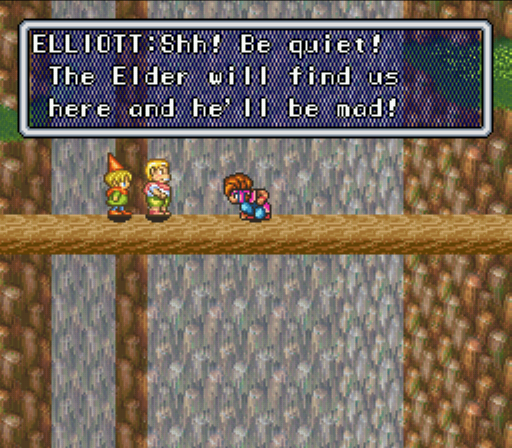
\includegraphics[scale=0.25]{install_chapter/pause1.png} {} 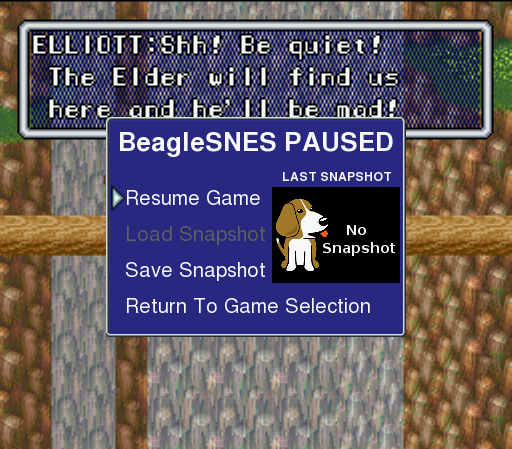
\includegraphics[scale=0.25]{install_chapter/pause2.png} {} 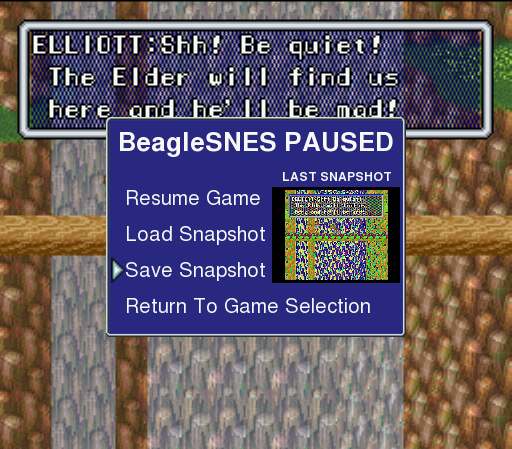
\includegraphics[scale=0.25]{install_chapter/pause3.png}
\caption{The pause menu.  While in-game (left), triggering the pause menu will bring up a set of menu options (middle). If a snapshot for the current game has been previously saved, the ``Load Snapshot'' option will become active and a thumbnail will be shown in the ``LAST SNAPSHOT'' preview window.}\label{fig:pause_menu}
\end{figure}

There are three ways to trigger the pause menu:
\begin{itemize}
\item If the pause menu has been mapped to a single gamepad button in \texttt{games.xml}, press that button. 
\item If a pause button combination has been mapped in \texttt{games.xml}, press that button combo.
\item If the pause menu has been mapped to a GPIO in \texttt{games.xml}, trigger that GPIO.
\end{itemize}

Pressing up and down on the player 1 gamepad, or triggering the appropriate GPIOs, will navigate the pause menu.  Likewise, using select/start or its GPIO equivalent will select a menu option. Selecting ``Resume Game'' will remove the pause menu and unpause the game.  Also, pressing the pause button or button combo, or triggering the pause GPIO, a second time will also remove the pause menu and unpause the game.

The ``Load Snapshot'' and ``Save Snapshot'' menu options allow you to save the current state of the game and then load it to return to it at any time. This is useful for saving the progress of the current play session when you need to take a break and are not near a point in the game where progress can be saved.  It is also useful for saving your game just prior to making that difficult jump or fighting a tough boss battle.  Snapshots are named after the filename of the ROM that they are associated with, so renaming ROMs will make your save states seem to disappear (although they are still present on the microSD card).  If no snapshot for the current game exists, the ``Load Snapshot'' option will be grayed-out and unavailable.  Only one snapshot can exist for each game.  Once a snapshot is saved, the prior snapshot is overwritten.

\begin{updateWarn}
Snapshots are stored in the \texttt{savestate} subdirectory of the \texttt{beaglesnes} directory on the \texttt{/boot} partition.
\end{updateWarn}

The ``Return to Game Selection'' menu option exits the current game and return you to the game selection menu. Be sure to save a snapshot of your current game if you want to return to it later.  Selecting this option is roughly the same as turning off the power on your SNES console: your current game will be lost forever.
  

%----------------------------------------------------------------------------------------
%	TROUBLESHOOTING CHAPTER
%----------------------------------------------------------------------------------------

\chapter{Troubleshooting}

\section{Overview}\index{Overview}

{\bf If you are unable to \texttt{dd} the full system image to your microSD card:}
\begin{itemize}
\item Do you not have \texttt{bunzip2} on your system?  For Ubuntu users, you can \texttt{apt-get} it by installing the \texttt{bzip2} package.
\item Is your download corrupt?  Does the MD5 hash for the file match the hash listed for the file at SourceForge? 
\item Did you disable the write-protect switch on your microSD card?
\item Do you have permissions to write to the raw microSD card device file?
\item Are any pre-existing partitions on the microSD card currently mounted?  Unmount all partitions on the microSD card before performing the \texttt{dd}. 
\end{itemize}

\noindent{}{\bf If you can't get your system to boot after writing the full system image to your microSD card:}

\begin{itemize}
\item Are you using an external power supply (5VDC 2A)?  The system won't boot when using only USB power.
\item Did you disable the write-protect switch on your microSD card?  The BeagleSNES still needs to write out log files to the local file system.
\item Is there any output coming from the debug serial or FTDI port? If there is nothing, \texttt{dd} the full file system to the microSD card again after you verify the MD5 hash of the downloaded file.
\item Did you cleanly unmount the microSD card from the Linux system that you used to \texttt{dd} the image to the card? Some Linux systems will auto-mount the microSD card as soon as it has a valid file system on it.  If you just pull the microSD card out when it is mounted, it is possible to damage the boot partition.
\item Did you change the boot configuration from the default BBB HDMI configuration if you needed to do so?  If you are using a BBxM, you will need to change the boot configuration to the BBxM configuration to use the proper bootloader.
\end{itemize}

\noindent{}{\bf If you can see the boot splash screen, but the emulator won't start:}

\begin{itemize}
\item If you revert to the backup of the original \texttt{games.xml} file (you made that backup, right?) does the emulator start?  If so, you have a mistake in your \texttt{games.xml} file.
\item If you do not see anything wrong with your \texttt{games.xml} file, does the debug output over serial or FTDI show any errors in parsing the XML? Any errors will give you hints as to where troubles may lie in your \texttt{games.xml}.
\item Make sure that all box image and ROM filenames are correct.  The filenames are case-sensitive, and you do not need to add the directories to the filenames.
\item If nothing else works, shell into the system via the network and try to manually execute the \texttt{service.sh} script in the application root directory.  You will need to \texttt{sudo} the command or be a superuser in order to do so.  Watch for any debug output that might give you a hint as to why it is not working.
\item If all else fails, send us a bug report and we'll check it out.
\end{itemize}

\noindent{}{\bf If the game selection menu appears, but it does not respond to your USB gamepad:}

\begin{itemize}
\item Do you have the Tomee USB gamepad?  If not, you may have to play with the button mappings in the \texttt{games.xml} file.
\item Is your gamepad plugged into the correct USB port?  Do you see the message telling you to plug in the "player one" gamepad?  Only a gamepad that is plugged into the "player one" USB port can control the menu selection screen.
\item For the BBB, there is a known kernel bug that causes USB devices to not be enumerated by the USB bus.  Press the "Reset" button (button S1) or unplug and plug in the power cable to reset the system and try again.  It may take a few tries, unfortunately.  Watch the FTDI output for an \emph{Error -110} to see if this is the particular problem that you are seeing.  This problem appears to occur less often once the system has been running for a while, and it may take several tries before the errors go away and the USB subsystem enumerates properly.
\item For the BBB, plugging an external USB hub into the host USB port can be very tempermental.  If using an external hub, plug in the hub and all controllers prior to starting the system.  Sometimes the external hub will stop responding if all controllers are removed from it.  An unpowered external hub will work, but it makes the BBB far more sensitive and can create problems when hotplugging controllers.
\item Verify that your gamepad is operating properly by testing it with another computer.  
\end{itemize}

\noindent{}{\bf If the game selection menu starts, but is missing one or more of your titles:}

\begin{itemize}
\item If you do not see anything wrong with your \texttt{games.xml} file, does the debug output over serial or FTDI show any errors in parsing the XML? Any errors will give you hints as to where troubles may lie in your \texttt{games.xml}.  
\item Did you use predefined entries in the XML for any special characters (Section~\ref{sec:games_xml})? Parsing of the XML will stop once an error is reached.
\end{itemize}

\noindent{}{\bf If the game selection menu starts, and you can launch a title, but then the screen goes blank and nothing happens:}

\begin{itemize}
\item Make sure the filename for the ROM is correct in the \texttt{games.xml} file.
\item Make sure that the ROM is valid by executing it under another emulator.
\item Make sure that the ROM is in the \texttt{rom} subdirectory of the \texttt{beaglesnes} directory in the \texttt{/boot} partition.
\end{itemize}

\begin{updateWarn}
If you run into some other problem that is not covered here, please feel free to submit a bug report to Andrew at \texttt{hendersa@icculus.org}.
\end{updateWarn}


%----------------------------------------------------------------------------------------
%	BUILDING CHAPTER
%----------------------------------------------------------------------------------------

\chapter{Building BeagleSNES}

\section{Overview}\index{Overview}

BeagleSNES is more than just a single application.  It is a complete operating system with a custom Linux kernel, a full file system, and configuration files that tell BeagleSNES how to behave for the end user.  Because of this, it can be sometimes be difficult to get up and running.  This section focuses on building the individual components of BeagleSNES using the build scripts that have been included to assist you.  Unless you are interested in installing/uninstalling/changing configurations/libraries/binaries in the file system, it is probably best to leave the file system as-is and concentrate on modifying only the bootloader, kernel, and BeagleSNES application.

\section{Bootloader}\index{Bootloader}

BeagleSNES's bootloader is a modified version of the v2014.01 release of U-Boot.  The BeagleSNES source code archive for the bootloader is just a \texttt{tar}'d-up version of the hacked-on, working code base of what is running inside of the BeagleSNES system.  Use the following steps to build it:

\begin{itemize}
\item Install a cross-compiler tool chain on your development system.  BeagleSNES's development was done using a tool chain built using \texttt{crosstool-ng}\footnote{Download \texttt{crosstool-ng} at: \texttt{http://crosstool-ng.org}}, though you could probably install an ARM development tool chain via \texttt{apt-get} or whatever package manager your particular Linux distribution is using.  It is also possible to use the tool chain that is included with the BeagleSNES kernel source.
\item Edit the \texttt{beaglesnes-build.sh} shell script in the \texttt{beaglesnes\_u-boot} code base to point to the location of your cross-compiler tool chain.  You'll need to modify the \texttt{TOOL\_PATH} and \texttt{TOOL\_CHAIN} variables to point to the path where your tool chain is located and the prefix of each tool chain binary, respectively.  \texttt{crosstool-ng} installs the tool chain in \texttt{\$(HOME)/x-tools}, so that will most likely be the value that you need to set for \texttt{TOOL\_PATH}.  Tool chain binaries are typically named following the format of \texttt{\$TARGET\_ARCH\$TOOL}.  \$TOOL is \texttt{gcc}, \texttt{g++}, etc., and \texttt{\$TARGET\_ARCH} is probably something similar to \texttt{arm-cortex\_a8-linux-gnueabi-}.
\item Edit the \texttt{beaglesnes-build.sh} shell script to choose to build the bootloader for the BB-xM or the BBB.  To do this, there are two lines in the shell script that build a configuration for \texttt{omap3\_beagle\_config} (BB-xM) and \texttt{am335x\_evm\_config} (BBB).  Uncomment only one of these two lines to select the hardware to build the bootloader for.  The comments in the shell script will guide you.    
\item Once you have set up your \texttt{beaglesnes-build.sh} script, execute it.  This will start the build process and generate a variety of files in the \texttt{beaglesnes\_u-boot} directory.  The two files that you are interested in are \texttt{MLO} (the first stage bootloader) and \texttt{u-boot.img} (the second stage bootloader that actually loads the kernel).  
\item Mount the first partition (the boot partition) of a microSD card that has had the full BeagleSNES file system image written to it.  \emph{Back up the \texttt{MLO} and \texttt{u-boot.img} binaries in the root of that mounted partition.} 
\item Replace the \texttt{MLO} and \texttt{u-boot.img} binaries on the microSD card (\emph{after you have backed them up}) with the \texttt{MLO} and \texttt{u-boot.img} that you just built.
\item \texttt{sync} the microSD card's mounted boot partition's file system, then unmount it.    
\end{itemize}

\noindent{}You've just built the BeagleSNES bootloader and installed it.  Insert the microSD card into the system, power it up, and it should now boot using your new bootloader.  Remember that your new bootloader files will be replaced with the stock BeagleSNES ones if you execute the \texttt{setup\_BBB.sh} or \texttt{setup\_BBxM.sh} scripts in the boot partition.

\section{Kernel}\index{Kernel}

BeagleSNES's BB-xM kernel is built from a snapshot of the Linux 3.7.10 kernel branch of Robert Nelson's stable kernel project\footnote{\texttt{https://github.com/RobertCNelson/stable-kernel}} that was retrieved using \texttt{git} on 11 March 2013.  The BBB kernel is built from a snapshot of the 3.8.13 kernel branch from the same project, retrieved on 02 June 2013.  Both of these projects contains a script called \texttt{build\_kernel.sh} that performs a number of useful activities:

\begin{itemize}
\item Installs a cross-compilation tool chain for building the kernel.
\item Checks for new kernel patches.
\item Applies kernel patches (over 200 of them!) to the kernel source tree for all BeagleBoard platforms.
\item Builds the kernel.
\end{itemize} 
 
\noindent{}The BeagleSNES kernel source trees contain the \texttt{build\_kernel.sh} file, but it has been modified.  The script no longer checks for kernel patches and updates or downloads the tool chain.  The tool chain is already present in the BeagleSNES kernel source package\footnote{The tool chain is in the \texttt{dl/gcc-linaro-arm-linux-gnueabihf-4.7-2012.12-201214\_linux} directory.}, so there is no need to download it again.  To build one of the kernels, use the following steps:

\begin{itemize}
\item \emph{Optional:} If you want to rebuild the splash screen that displays during kernel boot, execute the \texttt{build\_beagle\_splash.sh} script.  This will convert the splash screen image file\footnote{\texttt{beaglesnes\_kernel\_splash.png}} into the proper format and then copy it to its place in the kernel source tree.  Note that the splash screen image is different in the two kernel trees.  For BB-xM, it is 640x480.  For BBB, it is 720x480.
\item Execute the \texttt{build\_kernel.sh} script.
\item Choose to "Exit" the kernel configuration tool without changing any settings.  \emph{Note: Don't change the configuration unless you know what you are doing!}  The kernel will then begin building, which will take a few minutes.  All generated binaries will be under the \texttt{deploy} directory of the BeagleSNES kernel source.
\item Mount the first partition (the boot partition) of a microSD card that has had the full BeagleSNES file system image written to it.  \emph{Back up the \texttt{zImage} (BB-xM) or \texttt{3.8.13-bone20.zImage} kernel binary in the root of that mounted partition.} 
\item Replace the kernel binary on the microSD card (\emph{after you have backed it up}) with the \texttt{deploy/3.7.10-x9.uImage} or \texttt{deploy/3.8.13-bone20.zImage} kernel binary that you just built. Rename the \texttt{3.7.10-x9.uImage} kernel to \texttt{zImage} in the \texttt{/boot} partition.
\item \texttt{sync} the microSD card's mounted boot partition's file system, then unmount it. 
\end{itemize}

\noindent{}\emph{Optional:} The BeagleSNES does not load any kernel modules (everything necessary is built directly into the kernel), but if you also want to install the kernel modules created when the kernel is built, use the following steps (performing the commands using \texttt{sudo}):

\begin{itemize}
\item Mount the second partition (the rootfs partition) of a microSD card that has had the full BeagleSNES file system image written to it.  \emph{Back up the \texttt{/lib/modules/3.7.10-x9} (BB-xM) or \texttt{/lib/modules/3.8.13-bone20.zImage} (BBB) directory in the root of that mounted partition.} 
\item If building for a BB-xM, replace the \texttt{/lib/modules/3.7.10-x9} directory on the microSD card (\emph{after you have backed it up}) with the \texttt{deploy/mod/lib/modules/3.7.10-x9} directory that you just built.
\item If building for a BBB, copy the file \texttt{deploy/3.8.13-bone20-modules.tar.gz} to the \texttt{/lib/modules} directory on the microSD card. \texttt{gunzip} and un\texttt{tar} the file.  Replace the \texttt{/lib/modules/3.8.13-bone20} directory on the microSD card (\emph{after you have backed it up}) with the \texttt{/lib/modules/lib/modules/3.8.13-bone20} directory.
\item \texttt{sync} the microSD card's mounted rootfs partition's file system, then unmount it. 
\end{itemize}

\noindent{}You've just built the BeagleSNES kernel and installed it.  Insert the microSD card into the system, power it up, and it should now boot using your new kernel.

\emph{Advanced Users:} If you are interested in using the latest kernel source and patches, fetch the latest code from Robert Nelson's Git repository and replace the \texttt{.config} in the kernel source with the \texttt{beaglesnes\_config} file from the top-level directory of the BeagleSNES kernel source.  The \texttt{beaglesnes\_config} file is a copy of the kernel configuration that is used when building the BeagleSNES kernel.  It will ensure that you build a kernel with the proper features enabled.  By default, the kernel from Git tries to be generic as possible by building a \emph{large} number of hardware drivers as modules.  BeagleSNES does not build most of these drivers, and the ones that it does need are linked directly into the kernel, rather than being built as modules.

\section{BeagleSNES Application}\index{BeagleSNES Application}

The BeagleSNES application is both the game selection menu front-end and the SNES emulator back-end.  Both components are built as a single binary.  The application has the following library dependencies:

\begin{itemize}
\item The Simple DirectMedia Library\footnote{\texttt{http://www.libsdl.org}} for general audio, video, and input.
\item The SDL\_ttf library\footnote{\texttt{http://www.libsdl.org/projects/SDL\_ttf}} for rendering TrueType fonts.
\item The SDL\_image library\footnote{\texttt{http://www.libsdl.org/projects/SDL\_image}} for loading image files of various formats.
\item The SDL\_mixer library\footnote{\texttt{http://www.libsdl.org/projects/SDL\_mixer}} for loading and playing music and sound effects.
\item The Expat library\footnote{\texttt{http://expat.sourceforge.net}} for parsing the XML \texttt{games.xml} file.
\end{itemize}

\noindent{}Because it can be difficult to build and install all of these libraries correctly using a cross-compiler tool chain, it is easiest to build both the libraries and the BeagleSNES application on the BB-xM or BBB.  The BeagleSNES full system image contains all of these libraries and header files, as well as a complete development tool chain.  These instructions will assume that you are building BeagleSNES inside of the full system image.  

\begin{updateWarn}
If you decide to use a package manager (like \texttt{apt-get}) to install the needed libraries, you're going to drag in a number of additional dependencies that you won't need.  Typically, SDL is built with X11 support, so your package manager will install a large number of X-Windows applications and libraries.  It is better to build the libraries manually than to install them via a package manager.  If you don't have the patience or experience to manually install the libraries and their dependencies, stick with using the libraries and headers already installed in the full file system image.  These libraries include only the most basic features of SDL (framebuffer console graphics, ALSA audio, and the joystick input subsystem).
\end{updateWarn}

The BeagleSNES application source code is available as a downloadable source code archive.  The source code is also installed inside the full system image\footnote{It is in the \texttt{/home/ubuntu/build/beaglesnes\_src} directory within the full system image.}.  To build the BeagleSNES application on a BB-xM or BBB system, use the following steps:

\begin{itemize}
\item Shell into the running BeagleSNES system (username "ubuntu", password "temppwd").  The easiest way to do this is via the serial debug interface\footnote{Read \texttt{http://elinux.org/BeagleBoardFAQ} for more information on setting up and using the serial debug interface}, though you can also use \texttt{ssh} to shell into the system via the ethernet interface.
\item Enable swap space.  \texttt{swapfile} is a one gigabyte swap file that has already been created for you in the full system image.  You only need to turn on swapping by using the command: \texttt{sudo swapon /var/cache/swap/swapfile}
\item \texttt{cd} into the \texttt{/home/ubuntu/build/beaglesnes\_src/sdl} directory.
\item Execute the \texttt{configure} script in this directory.  The script should find the tool chain and all of the necessary libraries and headers to build the application.  For best performance, execute the \texttt{configure} script with the \texttt{-{}-enable-neon} option:
\begin{commandBox}
\texttt{ubuntu@beaglesnes\$  sudo ./configure -{}-enable-neon}
\end{commandBox}
\item Edit the \texttt{beagleboard.h} file to select which platform you are building for.  There are two \texttt{\#define} statements: one for \texttt{BEAGLEBONE\_BLACK} and one for \texttt{BEAGLEBOARD\_XM}. Uncomment the \texttt{\#define} that describes your system, and comment out the other one.
\item If you have chosen to enable the \texttt{BEAGLEBONE\_BLACK} build via \texttt{beagleboard.h}, you can also comment in the "\texttt{\#define CAPE\_LCD3 1}" in \texttt{beagleboard.h} to enable the support for the LCD3 display instead of the HDMI video output.
\item Execute a \texttt{make} command in this directory.  The application will now build, and it will take a while.  If you did not enable swapping, the system will exhaust its RAM and fail on this step.
\item \emph{Optional:} Shrink the generated binary (and reduce its loading time) by stripping it via the command: \texttt{strip ./snes9x-sdl}
\item Copy the generated \texttt{snes9x-sdl} binary to the \texttt{/home/ubuntu/beaglesnes} directory.  If you built a binary for BBB with HDMI video, name it \texttt{snes9x-sdl.BBB.HDMI}.  If you built a binary for BBB with HDMI video, name it \texttt{snes9x-sdl.BBB.LCD3}. If you built a binary for BB-xM, name it \texttt{snes9x-sdl.BBxM}.  These are the files that the \texttt{service.sh} script looks for.
\item Execute a \texttt{sync} command. 
\end{itemize}

%----------------------------------------------------------------------------------------
%	KERNEL/BOOTLOADER CHAPTER
%----------------------------------------------------------------------------------------

\chapter{BeagleSNES Kernel and Bootloader}

\section{Overview}\index{Overview}

BeagleSNES uses the U-Boot bootloader\footnote{\texttt{http://www.denx.de/wiki/U-Boot}} and a trimmed-down Linux kernel.  The configuration of both of these components impacts both the runtime performance of the system and the time necessary to boot the system.  A general timeline of the events that occur as the system boots is as follows:

\begin{table}[h]
\centering
\begin{tabular}{| l | l |} \hline
%\toprule
\textbf{Time (seconds)} & \textbf{Events Taking Place}\\ \hline
%\midrule
0 & System is powered up \\
& Bootloader begins executing immediately \\
& Bootloader fetches its configuration file from the boot partition \\ 
& Bootloader initializes DVI video at a resolution of 1280x720 (BB-xM)\\ \hline
2 & Bootloader has finished loading and decompressing the kernel \\
& Kernel begins bootstrapping \\ 
& Bootloader terminates execution \\ \hline
5 & Kernel initializes DVI video at a resolution of 640x480 (BB-xM) \\
& Kernel turns on framebuffer console (BB-xM) \\
& Boot splash screen is displayed (BB-xM) \\ \hline
8 & Kernel initializes HDMI video at a resolution of 720x480 (BBB) \\
& Kernel turns on framebuffer console (BBB) \\
& Boot splash screen is displayed (BBB) \\ 
& \texttt{init.sh} script in the BeagleSNES image is executed \\ \hline
10 & Boot splash screen disappears \\
& BeagleSNES is launched via the \texttt{service.sh} script \\
& Game selection menu logo and gradient bar appear on the screen \\ \hline
12 & Game selection menu displays entire screen and begins playing audio \\
& System is now accepting user input and is ready for use \\ \hline
%\bottomrule
\end{tabular}
\caption{Timeline of BeagleSNES events, from power up to "usable system".}
\end{table}

While waiting 12 seconds for an embedded system to achieve a usable state is still quite a long time, earlier development versions of BeagleSNES would take as long as \emph{35 seconds} to go from power up to usable system.  There is still room for a great deal of improvement in the boot speed of BeagleSNES.  Other projects, such as SwiftBeagle\footnote{\texttt{http://code.google.com/p/swiftbeagle/}}, have done an excellent job discovering various ways that the bootloader and kernel can be changed in order to decrease boot time.  In this section, several of these points will be discussed as the bootloader and kernel of BeagleSNES are examined.

\section{Bootloader}\index{Bootloader}

BeagleSNES's U-Boot bootloader has had two noteworthy modifications: the standard 3-second delay prior to loading the kernel has been removed\footnote{This setting is located in the file \texttt{include/configs/omap3\_beagle.h} (BB-xM) and \texttt{include/configs/am335x\_evm.h} (BBB) in the bootloader source.  It is the \texttt{CONFIG\_BOOTDELAY} pre-processor define.} and preliminary support has been added for a bootloader splash screen\footnote{These modifications have been added to the file \texttt{board/ti/beagle/beagle.c} in the bootloader source.  Check out \texttt{dss\_init()}, which sets up the memory buffer and does some register adjustments.} for the BB-xM.  Version 2013.04 (used in BeagleSNES v0.4) is the earliest version of U-Boot that will work for BeagleSNES because it is the first version to include \emph{device tree} support\footnote{To learn more about the device tree and how it is used in the Linux kernel to describe hardware peripherals for embedded devices, go to \texttt{http://www.devicetree.org}} for the BBB's cape bus.  

A BeagleSNES bootloader configuration file, \texttt{uEnv.txt}, exists for the BB-xM and both BBB boot configurations.  Each of the uEnv.txt files set a U-Boot environment variable called \texttt{bootargs}.  This value of this variable is the set of command line arguments that are passed to the Linux kernel when the kernel begins its bootstrapping process.  There are two sets of \texttt{bootargs} in each of the \texttt{uEnv.txt} files: one for a quicker-booting configuration that specifies the BeagleSNES \texttt{init.sh} script as the "init" process for the Linux kernel, and one for a slower-booting configuration that uses the default Linux \texttt{systemd}\footnote{To learn more about \texttt{systemd} and its role as a system and service manager for Linux, go to \texttt{http://www.freedesktop.org/wiki/Software/systemd}}  as the "init" process.  By default, the "fast boot" configuration is enabled, which enables BeagleSNES to get up and running as quickly as possible.

The quicker-booting configuration allows the system to boot in about half of the time it takes the slower-booting configuration.  This is because the quicker configuration does not start many of the system daemons that are started in the slower configuration (since \texttt{systemd} is not used and the usual init scripts are not executed).  The quicker configuration performs only the bare minimum of remounting the root filesystem read-write, starting \texttt{udevd} (to create the device files for the USB gamepads in the \texttt{/dev} filesystem), and adjusting the ALSA mixer levels.  The downside to this is that many other important services, such as networking, are never started.  Aside from the difference in the "init" process that is used, both configurations for each platform specify \texttt{bootargs} that turn on debug output to the serial port, enable the DVI or HDMI video output at specific resolutions, and shut off the framebuffer's blinking cursor.

\emph{Switching between the faster and slower boot configurations requires editing the \texttt{uEnv.txt} file.} The \texttt{bootargs} for both configurations are in each of the \texttt{uEnv.txt} files, so it is only a matter of commenting out the configuration that isn't needed and commenting in the configuration that is.  Make sure that only one configuration is commented in at a time.  Comments have been included in the \texttt{uEnv.txt} files to guide you.  The \texttt{uEnv.txt} files that come with BeagleSNES can be seen in Figures~\ref{fig:BBxM_uEnv} (for the BB-xM), \ref{fig:BBB-HDMI_uEnv} (for the BBB with HDMI), and \ref{fig:BBB-LCD3_uEnv} (for the BBB with LCD3).

\begin{figure}[h]
\lstinputlisting{BBxMuEnv.txt}
\caption{BeagleSNES's BB-xM \texttt{uEnv.txt} bootloader configuration file.}\label{fig:BBxM_uEnv}
\end{figure}
\begin{figure}[h]
\lstinputlisting{BBB-HDMI-uEnv.txt}
\caption{BeagleSNES's BBB HDMI \texttt{uEnv.txt} bootloader configuration file.}\label{fig:BBB-HDMI_uEnv}
\end{figure}
\begin{figure}[h]
\lstinputlisting{BBB-LCD3-uEnv.txt}
\caption{BeagleSNES's BBB LCD3\texttt{uEnv.txt} bootloader configuration file.}\label{fig:BBB-LCD3_uEnv}
\end{figure}

\section{BeagleBoard-xM Kernel}\index{BeagleBoard-xM Kernel}

BeagleSNES was originally developed specifically for the Rev C BB-xM. While the Linux kernel has good support for the BB-xM hardware (OMAP3, TWL4030, etc.), every embedded system kernel must be tuned and patched for the specific environment in which it will be deployed.  The BeagleBoard platforms are no exception.  BeagleSNES's kernel codebase uses a series of 207 kernel patches that have been contributed and vetted by the BB community.  While not every patch is specific to the BB-xM (BeagleBoard- and BeagleBone-specific patches are also applied), many of the patches increase system stability by improving voltage core management and thermal management.

The kernel itself has been compiled to remove many features that aren't needed for BeagleSNES.  This has reduced the compressed size of the kernel from 3.4 megabytes with additional modules dynamically loaded down to a little less than two megabytes with no additional modules loaded.  While this might not seem like a big difference, it has reduced the boot time of BeagleSNES by about 6 seconds.  Roughly 200 ms of these savings are attributed to the reduction in time needed to load and decompress the smaller kernel.  The bulk of the savings comes from eliminating the time needed to initialize various kernel subsystems that are never be used.  For example, many security features (SELinux, address space layout randomization (ASLR), stack overflow protection), symmetrical multi-processing support, support for various file system types, SCSI support, etc. were all originally compiled into the kernel. 

The BB-xM's DM3730 CPU begins running at a clock speed of 600 MHz, but is quickly changed to 800 MHz per the \texttt{mpurate} kernel command line option that is provided by the bootloader.  The "performance" governor\footnote{Option \texttt{CPU Power Management} -> \texttt{CPU Frequency scaling} in the kernel configuration menu.} forces the CPU clock rate to remain at its maximum rate of 800 MHz.  Originally, \texttt{mpurate} was set to "auto" and the "ondemand" governor was used by the kernel.  The high CPU utilization of the emulator would force the governor to adjust the clock speed from 600 MHz to 800 MHz once the BeagleSNES application began executing in user space.  This caused the system to boot more slowly (since the CPU clock was at 600 MHz for the entire kernel bootstrap process), so the \texttt{mpurate} and governor were changed accordingly.   

While this CPU can theoretically be clocked at 1GHz, there are a few problems with doing so. The BeagleSNES kernel source lacks a patchset that existed in earlier kernel versions (2.6.36, 3.0) that handle the VDD1 voltage adjustment of the CPU. It is non-trivial to port this patch set to newer kernels. While the clock speed could be forced to 1GHz without this patch set, you will slowly fry your BB-xM's CPU while doing so. The system also becomes a bit unstable when you're pushing the CPU at 100\% at 1GHz, which leads to application crashes (including BeagleSNES). Therefore, the governor will only push the clock speed to a stable 800 MHz.

\emph{An interesting note:} Titles that use Super FX\footnote{For more information on Super FX, refer to the Wikipedia article: \texttt{http://en.wikipedia.org/wiki/Super\_fx}} chips, such as "Star Fox", run really well when the system is clocked to 1GHz (5 FPS at 800 MHz versus 20-25 FPS at 1 GHz). The extra clock speed does make a big difference.

\section{BeagleBone Black Kernel}\index{BeagleBone Black Kernel}

When the BBB was first released in April 2013, the 3.8 Linux kernel was the OS kernel for the board.  The BBB's kernel branch consisted of the mainline 3.8 kernel source tree with hundreds of patches applied to it to support the BBB's functionality.  While the BBB's hardware is largely based upon that of its predecessor, the BeagleBone, the BBB's 3.8 kernel is quite different from the mature 3.2 kernel used by the BeagleBone.  Thus, the change from 3.2 to 3.8 for BBB led to new kernel features and new problems.

The main advantage of using the new 3.8 kernel was the introduction of the Device Tree\footnote{Learn more about the Device Tree at \texttt{http://www.devicetree.org/Main\_Page}.} data structure. This data structure allows for a more-uniform way of defining processor pin multiplexing ("muxing"), identifying which kernel resources and drivers are associated with particular processor pins.  Unfortunately, the 3.8 kernel is a combination of different kernel subsystems and can be a bit tempermental at times.  BeagleSNES will be moving to the 3.12/3.13 kernel tree once more testing has been completed and BeagleSNES is properly adapted to use it.  Other than the newer features of the 3.8 kernel, the BBB's kernel is quite similar in nature to that of the BBxM: the "performance" CPU governor is used and the kernel has been trimmed down to reduce the kernel size, eliminate unneeded device drivers, and shorten kernel boot time.

\section{Other Improvements to Boot Speed}\index{Other Improvements to Boot Speed}

Other system customizations that contributed to a faster boot time are:

\begin{itemize}
\item Shrinking the size of the root file system partition from 7.5 gigabytes to about 3.5 gigabytes.  This reduces the file system mount time at system start up.
\item Shutting off unneeded daemons.  By default, the Ubuntu Linux image that BeagleSNES is based on started standard daemons like the print spooler, Apache web server, lvm, dns-clean, fetchmail, etc..  These daemons slow down system start up and use the CPU for no purpose.
\item Reducing the number of \texttt{tty} terminals.  There is no need for a dozen terminals on an embedded device, and it takes time and resources to start and maintain them all.
\end{itemize}

For further performance improvements, the place to begin is the removal of even more daemons.  The next place would be to remove unneeded files from the root file system, convert chunks of the remaining file system into read-only \texttt{cramfs} files, and then mount them to form a mostly read-only file system.  This will greatly reduce the portion of the file system that actually needs to be read-write (such as \texttt{/dev}, \texttt{/sys}, \texttt{/tmp}, etc.).  Moving to a lightweight shell, such as busybox\footnote{\texttt{http://www.busybox.net/}}, would allow for even more files to be removed.  

The BeagleSNES menu and emulator are currently built in-place on the BB-xM and BBB platforms, so a complete toolchain and debugger are installed inside of the current BeagleSNES image for convenience.  These tools could also be removed to reduce the size of the system even further.  The 1 gigabyte swap file could also be removed, saving a great deal of space.

%----------------------------------------------------------------------------------------
%	VIDEO, AUDIO, INPUT CHAPTER
%----------------------------------------------------------------------------------------

\chapter{BeagleSNES Subsystems}

\section{Overview}\index{Overview}

\begin{updateWarn}
This section is currently BB-xM only.  It must be rewritten to include BBB information.  The overall concepts are still the same, though.
\end{updateWarn}

BeagleSNES uses the Simple DirectMedia Layer (SDL)\footnote{\texttt{http://www.libsdl.org}} library to provide audio, video, and input event functionality for both the game selection menu and the emulator.  SDL is a cross-platform library which has a simple programming interface that abstracts away many of the details involved when creating multimedia applications.  The BeagleSNES emulator is based on an SDL port of SNES9X\footnote{The original SNES9X-SDL source, prior to the BeagleSNES modifications, can be fetched from the Git repository at: \texttt{https://github.com/domaemon/snes9x-sdl}}.  The mainline version of SNES9X only supports an X11 video display target, which is unsuitable for the framebuffer video of BeagleSNES.  By using the SDL port, BeagleSNES is able to support a variety of interfaces, including those offered by the the BB-xM platform.

While the game selection menu and the emulator are really two separate applications (after all, the only purpose of the game selection menu is to provide the emulator with the filename of the ROM to be loaded), both exist in the same binary.  Early testing showed that there was a visible screen flicker and a delay of several seconds when transitioning from one to the other when each was broken out as a separate binary.  Therefore, the game selection menu will initialize all of the needed SDL subsystems (audio, video, and joystick), execute, and then shut down the audio and joystick subsystems prior to transitioning to the emulator.  The emulator will then reinitialize the audio and joystick subsystems while leaving the video subsystem alone\footnote{SDL allows an application to change the video resolution on-the-fly without reinitializing the video subsystem.  When the game selection menu and the emulator used to use different screen resolutions, the emulator had to change the resolution when it began executing.  But, it did not need to restart the video subsystem to do so.}.  By not shutting down the video subsystem and reinitializing it, the visible screen flicker is removed.
 
\section{Audio Subsystem}\index{Audio Subsystem}

The BeagleSNES audio subsystem uses the ALSA\footnote{The Advanced Linux Sound Architecture.  Read more about it at: \texttt{http://www.alsa-project.org}} interface that is exposed by kernel.  The interface is provided by the system-on-chip (SoC) audio driver for boards that have TWL4030 audio CODEC hardware\footnote{This audio driver is located in the file \texttt{sound/soc/omap/omap-twl4030.c} in the kernel source tree.}.  SDL offers an ALSA back-end, so many of the details involved in interfacing with ALSA are abstracted away from BeagleSNES by SDL. 

The game selection menu uses a helper library, SDL\_mixer\footnote{\texttt{http://www.libsdl.org/projects/SDL\_mixer}}, to provide an even simpler interface to SDL's audio subsystem.  SDL\_mixer allows BeagleSNES to easily fade music in and out, load audio in a variety of formats, and mix several channels of audio together.  SDL only provides a standard interface for pushing audio data out to the audio driver back-end, so the more advanced functionality of SDL\_mixer provides the additional features needed to create a full-featured audio solution.

BeagleSNES configures the audio hardware of the BB-xM to use signed 16-bit stereo audio samples with a sampling rate of 32000 Hz.  Both the game selection menu and the emulator use these same audio settings for simplicity.  The audio subsystem is initialized in the game selection menu so that audio feedback and background music\footnote{The background music that is played behind the menu comes from the group ViRiLiTY.  It was originally the tracked background music of an illicit serial number generator used for the piracy of the "ALO Power Audio Converter" software.} can be played while the end-user examines the list of games that are available for play.  

When a game is launched from the menu, any playing audio fades out and the audio subsystem is shut down.  The emulator then reinitializes the audio subsystem using its original program logic.  The emulator's implementation of the SNES's audio DSP performs all of the audio mixing, so SDL\_mixer is no longer needed.  While the real SNES hardware will play audio at almost the same time that its DSP generates the audio data, the BeagleSNES emulator has audio latency of approximately 100 ms.  This is caused by the time needed to place the generated DSP audio into the kernel's circular audio buffer and the time needed before the pre-existing audio data ahead of the new data in the buffer is consumed.  In practice, this delay is hardly ever noticed.  This latency can be reduced by shrinking the size of the kernel audio buffer (12000 bytes), but this increases the amount of CPU resources dedicated to refilling the buffer and risks the possibility of an audio buffer underrun.


\section{Video Subsystem}

BeagleSNES system's video output is displayed via the BB-xM's DVI digital output.  The initial release of BeagleSNES used the S-Video analog output for NTSC video output, but this ended up being a poor choice for the following reasons: 

\begin{itemize}
\item The analog video signal is very noisy.  The horizontal sync varies from scanline to scanline, there is a lot of static, and the color quality is poor.  Whether this is due to poor drivers or poor hardware quality is unknown.
 \item The 720x482 NTSC resolution is larger than what is needed for BeagleSNES.  This means that more pixels are being updated than are actually needed, which degrades performance.
\item During development, profiling of BeagleSNES showed that displaying the framebuffer was much slower for the analog output than it was for the digital output.
\item The NTSC analog output has a refresh rate of 29.97 Hz, while the DVI digital output has a refresh rate of 60 Hz.  This means that the digital output can potentially display at a rate of 60 FPS, while the analog signal artificially limits the frame rate to half that amount.
\item NTSC signals suffer from overscan.
\end{itemize}

\noindent{}All components of BeagleSNES render their graphics to the framebuffer console, which is set to a native resolution of 640x480 and a color depth of 16 BPP.  These particular settings are hard-coded into the "omapfb" framebuffer driver\footnote{This framebuffer video driver is located in the file \texttt{drivers/video/omap/omapfb\_main.c} in the kernel source tree.} within BeagleSNES's Linux kernel. The refresh rate of 60 Hz means that whatever data is present in the framebuffer is pushed out as a single frame of video and is displayed for roughly 0.0167 seconds.  At the end of that time period, the data in the framebuffer will then be pushed out as the next single frame of video.

The emulator runs at a logical 60 FPS internally, but this does not necessarily mean that it will render video at 60 FPS.  The emulator can potentially skip the rendering of many frames of video if it falls behind schedule and needs to make up the difference.  The skipped frames will not even be noticed in many cases, though performance-intensive titles that require a large amount of CPU time to emulate the SNES hardware will not have enough CPU time left to perform the rendering of enough frames each second to make the gameplay "smooth".

\subsection{Video During Boot}\index{Video Subsystem}

One of the defining characteristics of a consumer-oriented embedded device is that it "turns on" immediately after it is powered up.  The device must give the consumer some indication that it is now going through its start-up process.  Displaying some sort of graphical splash screen immediately after power up is an excellent way to achieve this.  Unfortunately, BeagleSNES does not provide such a splash screen.  Or, at least, it does not do so immediately upon powering up.  To do so would require adding functionality to the BeagleSNES bootloader to display the splash screen\footnote{There actually is preliminary support for a splash screen in the bootloader, but it has not been "hooked up" yet and needs further testing.}. 

Roughly five seconds after power up, a much simpler method to display a splash screen becomes available.  At that point in time, the bootloader has loaded, decompressed, and begun bootstrapping the kernel.  The kernel initializes the graphical framebuffer and displays the first graphical output of the system: an 80x80 pixel, 224 color image of Tux the Penguin.  This icon is displayed in the upper left corner of the framebuffer console.  BeagleSNES turns this image into a splash screen by replacing the original image\footnote{This image is located at \texttt{drivers/video/logo/logo\_linux\_clut224.ppm} in the kernel source tree.} with a much larger image: a 640x480 pixel, 224 color image of the BeagleSNES logo.

\begin{figure}[h]
\centering
\includegraphics[scale=0.28]{video_chapter/boot_splash.png} 
\includegraphics[scale=0.28]{video_chapter/beaglesnes_kernel_splash.png}
\caption{The original BeagleSNES's splash screen (left) was the smallest size it could be (640x300) for NTSC (720x482), but the current one (right) is the same size as the screen resolution (640x480) for simplicity.}
\end{figure}

Even though BeagleSNES uses a full-screen splash image, it is not really necessary for the splash screen to be the full resolution of the screen.  The background color of the framebuffer is black, and the image is displayed in the upper left corner of the screen, so it is only necessary to include the bare minimum amount of splash screen image needed to center the BeagleSNES logo on the screen.  The splash screen is compiled into the kernel, so a smaller image reduces both the size of the kernel and the time it takes for the bootloader to load the kernel into memory from the microSD card.  Adding a splash screen in this fashion increases the compressed kernel's size by only about 20kb.  Normally, debug and information messages are printed to the framebuffer console as the kernel boots, but BeagleSNES suppresses the printing of these messages\footnote{These messages can still be viewed via the serial debug interface (\texttt{/dev/ttyO2}), though.} so that they do not overwrite the splash screen image.

The splash screen remains on the screen while the kernel continues to bootstrap.  Once it is finished, the splash screen disappears as the "icon" in the upper left corner is removed.  The screen remains blank until the game selection menu appears approximately 17-18 seconds after power-up.
 
\subsection{Game Selection Menu}\index{Video Subsystem}

The BeagleSNES game selection menu uses the entire 640x480 screen. The video subsystem of SDL is used to request an SDL video surface to render to.  This surface is not requested using the SDL\_FULLSCREEN flag, even though the resolution we want to use is the entirety of the screen.  Profiling the use of SDL\_FULLSCREEN has shown that it is much slower than not using it, so it is always better for BeagleSNES to use a "windowed" mode for all of its framebuffer graphics.  For the simple animations of the menu, though, the impact of slower execution is minimal.

When BeagleSNES used analog video, not all of the space on the screen was usable. Due to NTSC overscan, some portion of the edges of the screen may be "cut off" by the television that the image is being displayed on. The amount that is cut off varies depending upon the particular television, so it is important to design the interface so that there is a "safety buffer" around the edges of the screen where text and other important items must not be placed.  Typically, no more than a few pixels are cut off on each edge, though the left edge of the screen loses far more: a cut off of 12-16 pixels is common.  Digital video does not have this issue.

\begin{figure}[h]
\centering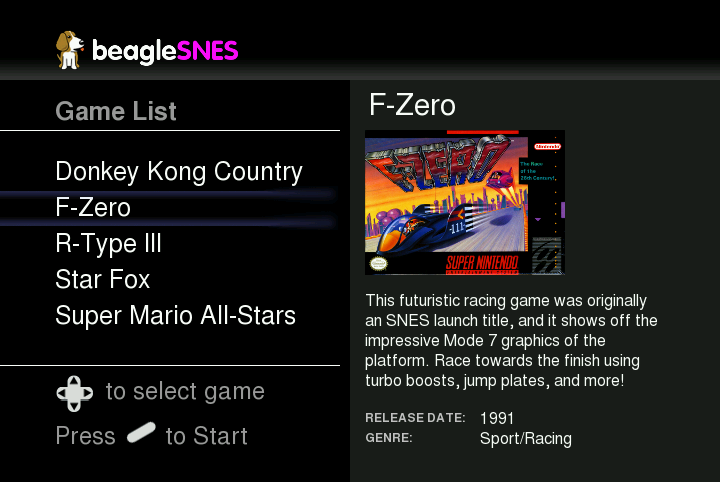
\includegraphics[scale=0.28]{video_chapter/gui_no_overscan.png} 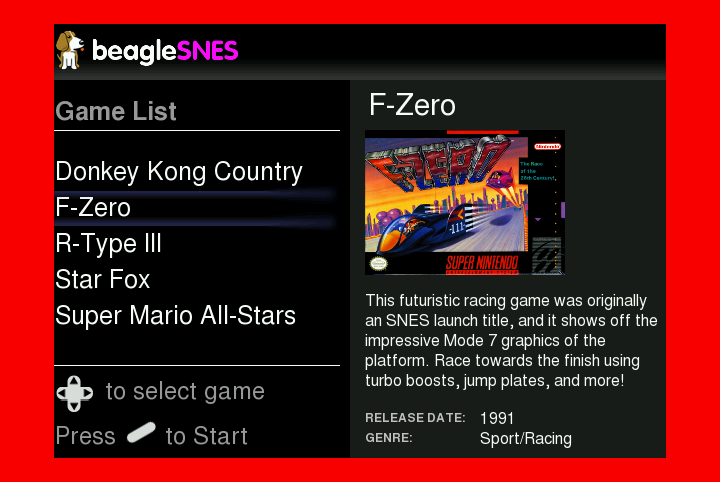
\includegraphics[scale=0.28]{video_chapter/gui_overscan.png}
\caption{A screenshot of the old game selection menu (left), and the same menu with the potential NTSC overscan regions marked in red (right).}
\end{figure}

\subsection{Emulator Execution}\index{Video Subsystem}

\emph{NOTE:} This section contains information about the video of the emulator from when BeagleSNES used analog video output.  It remains in the documentation because it may be of some technical interest to other BeagleBoard developers.

\emph{<Analog video material begins here>}

Once a selection has been made via the game selection menu, the screen fades to black prior to starting the emulator. This was not a choice based upon aesthetics (well, not directly, anyway). Internally, the emulator requests a 616x478x16 SDL video surface to render to. This resolution is different than what was previously set, so the SDL video subsystem actually has to be reconfigured with the new resolution. If the framebuffer is completely black, the transition between resolutions is never noticed by the end user. It also ensures that portions of the screen that are never updated by the emulator's rendering remain black during its execution.

The odd 616x478 resolution of the emulator was determined by the following method. Internally, each rendered scanline of SNES graphics is 512 pixels long. If we subtract the 512 pixels from the 720 pixel screen width, we have 208 pixels left in each scanline of the screen framebuffer (the screen framebuffer has a pitch of 1440 bytes, or (720 pixels * 2 bytes), so there are no extra offscreen pixels). If we divide these 208 pixels in half (since half will fall to the left of our SNES data and half will fall to the right of it), we have 104 pixels. 512 pixels + 104 pixels = 616 pixels, which is the resolution we request. Since we are not requesting a full-screen SDL video mode (via the SDL\_FULLSCREEN flag when calling SDL\_SetVideoMode()), the SDL surface will render into the left-most 616 pixels of the screen. With the offset of 104 pixels, the 512 pixels of the SNES scanline will render in the center of the screen. The emulator renders at a vertical resolution of 478 pixels. It is actually rendering each of the SNES's internal 239 scanlines twice to pixel double up to 478 scanlines. The SDL surface will render into the top-most 478 pixels of the screen, leaving the bottom 4 scanlines of the framebuffer untouched. Some, if not all, of these 4 scanlines will never even be seen, since they are usually lost to overscan.

\emph{<Analog video material ends here>}

Finally, by using an SDL\_UpdateRect() call to only update the portion of the framebuffer containing the 512x478 portion of SNES image data, we leave the chunks of black in the framebuffer that are to the left and right of the SNES graphics untouched. Why go to all of this trouble? Speed. There is a considerable difference between the speed of using the SDL\_FULLSCREEN mode (slow) and using only a portion of the screen (much faster). Titles that would run at close to 30 FPS would drop to 8-12 FPS when running in a full screen mode.

\section{Input Subsystem}\index{Input Subsystem}

BeagleSNES uses USB gamepad events as its only method for receiving input from the end user.  Both SDL and the Linux kernel view these gamepads as a USB human interface device (HID) class joystick devices.  SDL's input event mechanism for gamepads is split over two subsystems: video and joystick.  The video subsystem captures most events that are experienced by SDL-based applications: keyboard, mouse, window manager, etc..  Once the video subsystem is initialized, SDL's internal event queue is initialized as well.  Joystick events (the type of event that would be received from a gamepad) are an optional addition to the SDL event mechanism.  They are not received by the general SDL event handling code until the joystick subsystem is initialized.  Once that initialization occurs, gamepad events are also generated and placed into SDL's event queue alongside the other types of events.  

When the joystick subsystem is initialized, the underlying limitations of the Linux kernel's joystick interface become apparent.  The number of connected joysticks is reported, and any reported joysticks can then be "opened" to begin receiving events from them.  Unfortunately, there are \emph{many} things that could go wrong:

\begin{itemize}
\item If the USB hardware is unreliable (connections to devices are lost, but then quickly restored), SDL will stop responding to it.  This is because the "old" joystick is gone, but a "new" one has taken its place, and the new joystick must then be opened to use it.  
\item Joystick devices vary in the number of axis and buttons that the device provides to the software.  If an end-user plugs in a USB joystick device that reports a different number of buttons or axes, or reports buttons that are mapped in a different order than expected, then the behavior of the device will not be correct.
\item There are no "new joystick plugged in" or "joystick unplugged" events generated by SDL. There is only a mechanism to query how many joystick devices are currently plugged into the system.
\end{itemize}
 
BeagleSNES does its best to work around these limitations.  There is a known problem that the BB-xM has with briefly losing power to its USB devices.  This problem has the same effect as rapidly unplugging and then plugging in a gamepad: the gamepad appears to stop working because the joystick driver device file in the file system that SDL listens to for joystick events becomes invalid.   BeagleSNES addresses this problem with a kernel patch\footnote{This patch is for 3.2+ kernels.  Older kernels still suffer from this issue.} that properly handles this issue. 

Originally, BeagleSNES required that all gamepads must be plugged in prior to power up and not removed during system operation.  This situation is far from ideal, since gamepads can accidentally become unplugged during use.  The current approach to this problem is to tie the internal representation of a particular gamepad to the physical USB port on the system that the gamepad is plugged into.  Two of the BB-xM USB ports are designated explicitly for BeagleSNES gamepad use: one being the port for "player one" gamepad and the other for "player two".  Unless a gamepad is plugged into either of those particular ports (i.e. the "player one" or "player two" port), it will be completely ignored.  

When a USB gamepad is plugged into the BB-xM, new files are dynamically created in the \texttt{/sys} and \texttt{/dev} directories of the root file system, thanks to the \texttt{sysfs} support in the kernel\footnote{\texttt{sysfs} is a virtual file system that is accessible from user space.  It exports information about devices that are registered with the kernel, as well as a variety of driver information.  By reading these files from user space applications, the devices that these files represent can be interacted with easily.}.  Plugging a USB gamepad into the "player one" port creates a file\footnote{\texttt{/dev/input/by-path/platform-ehci-omap.0-usb-0:2.2:1.0-joystick}}, as does plugging a USB gamepad into the "player two" port\footnote{\texttt{/dev/input/by-path/platform-ehci-omap.0-usb-0:2.4:1.0-joystick}}.  Each of these files is a symbolic link to one of the \texttt{/dev/input/jsX} joystick device files.  These device files are opened from user space applications to access joystick events. By watching the creation and destruction of these files via a \texttt{stat()} or \texttt{readlink()} function call, BeagleSNES can determine whether a gamepad is present or not in those particular physical USB ports.  

The \texttt{/dev/input/jsX} device files enumerate the various joystick devices that are connected to the system, in the order that they are connected, using the device files \texttt{js0}, then \texttt{js1}, etc.  BeagleSNES will dynamically remap joystick events so that the events are attributed to the correct gamepad.  On each pass through the event handler loop, the "player one" and "player two" \texttt{sysfs} files are examined to see if they exist.  If either has changed, the joystick subsystem of SDL is shut down and restarted to reconfigure the gamepads accordingly.  This expensive operation only occurs if a controller has been plugged in or unplugged.  Otherwise, the only overhead created is by the two checks to see if the \texttt{sysfs} files exist and a table lookup to remap joystick events to the correct gamepad as those events occur.

  
%----------------------------------------------------------------------------------------
%	PORTABLE CHAPTER
%----------------------------------------------------------------------------------------

\chapter{Making BeagleSNES Portable}

\section{Overview}\index{Overview}

With the small physical size and flexibility of the BeagleBone family of boards, it is natural to consider using BeagleSNES as the software to drive a portable video game system.  To this end, some research has gone into developing such a system and has resulted in the new LCD3 cape display target for BeagleSNES. A prototype portable unit is shown in Figure~\ref{fig:full_unit}.
 
\begin{figure}[h]
\centering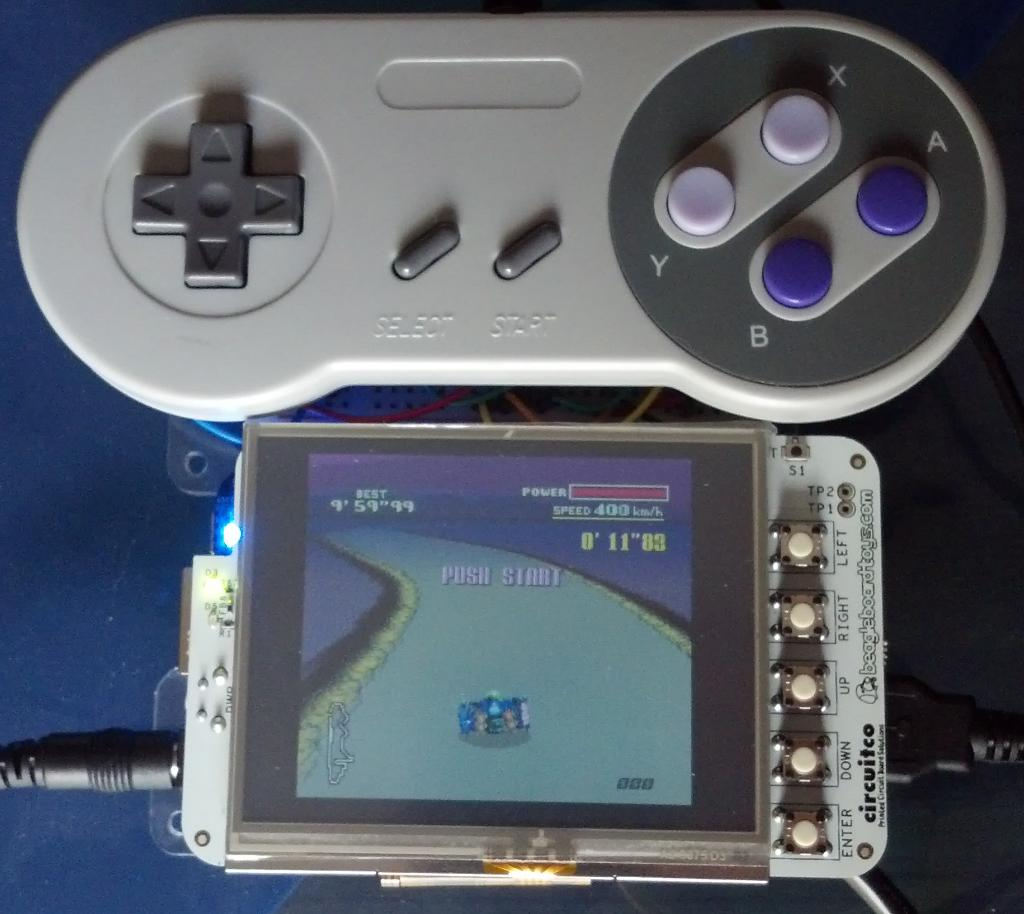
\includegraphics[scale=0.32,clip=true,trim=0 0 0 0]{portable_chapter/full_unit.jpg} 
\caption{A prototype of a portable BeagleSNES system. This prototype still requires a USB gamepad and power via the +5VDC barrel connector, so it isn't fully "portable".}\label{fig:full_unit}
\end{figure}

This target varies from the existing BBB target in the following ways:
\begin{itemize}
\item The LCD3 cape has a resolution of 320x240.  This requires a rework of the BeagleSNES front-end GUI.  On the bright side, such a small resolution allows the emulator to render at the native 256x239 SNES resolution without requiring the use of a software-based pixel-doubler to scale the SNES video output to the higher-resolutions used by the BBB and BB-xM.
\item Additional audio hardware is needed.  For the BBB HDMI target, a dummy CODEC in the kernel provides an ALSA interface to userspace.  Audio data written to the dummy CODEC is passed to the HDMI framer chip in I2S format.  The framer then packages up the audio data and sends it to the display via the HDMI protocol.  When not using the HDMI framer chip, a different audio device must be provided.
\end{itemize}

\section{Video}\index{Video}

The LCD3 cape, seen in Figure~\ref{fig:LCD3}, provides the video display functionality for a portable target.  It weighs approximately 70 grams and has a current consumption of 100mA.  While it is possible to use a smaller display, or at least a display module that has a smaller footprint, the easy availability and pre-packaged nature of the LCD3 cape makes it appealing for quick prototyping without having to worry about device drivers.  

\begin{figure}[h]
\centering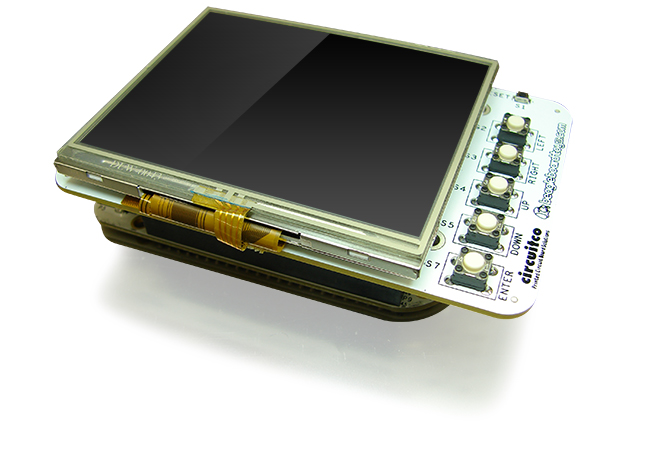
\includegraphics[scale=0.35,clip=true,trim=30 125 30 0]{portable_chapter/LCD3-Front.jpg} 
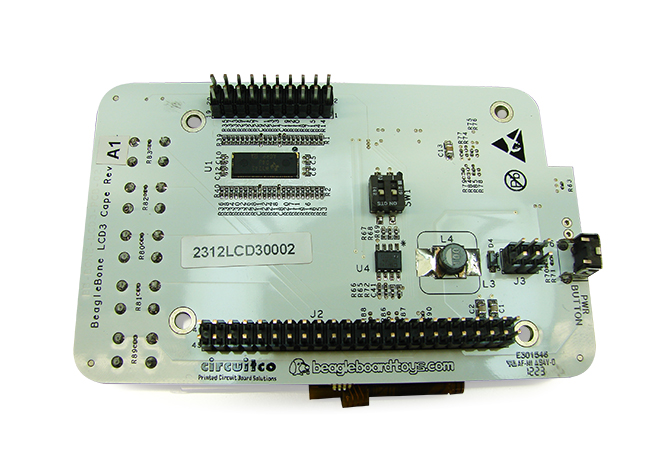
\includegraphics[scale=0.3,clip=true,trim=10 20 15 27]{portable_chapter/LCD3-Bottom.jpg} 
\caption{The LCD3 cape board made by CircuitCo. This 320x240 LCD has a touchscreen and five input buttons (left), and it plugs into the BBB's P8/P9 connectors via pins on the underside of the cape board (right). Photo credit: \texttt{http://elinux.org/CircuitCo:BeagleBone\_LCD3}}\label{fig:LCD3}
\end{figure}

Because the LCD3 cape is defined in the default Device Tree for the BeagleSNES kernel, it will be automatically detected and configured when it is connected to the BBB. The LCD3 uses the \texttt{TILCDC} driver in the kernel to provide a 16 BPP data bus between the BBB and the LCD3 cape.  This is the same driver that is used to communicate with the built-in HDMI cape of the BBB, so userspace software need not be aware of the differences between communicating with the LCD3 cape versus communicating with the HDMI framer chip on the HDMI cape.  As long as the 320x240 resolution is configured as a valid framebuffer resolution (by adding the appropriate framebuffer mode to the \texttt{/etc/fb.modes} file), BeagleSNES can simply request a 320x240 resolution and then adjust its rendering accordingly to use the LCD3 cape.   

\ignore{BeagleSNES makes use of the input features of the LCD3 cape.  The touchscreen is used to adjust the volume of the unit.  Touching the left side of the display will decrease the volume and touching the right side will increase it.  Overlay bars will appear to let you know what the current volume level is whenever the volume has been changed, but they will disappear once there have been no changes in volume change within the last X seconds.  The input buttons on the side of the display are mapped to the up/down/left/right directional pad of the first gamepad, so the game selection GUI can be navigated by using them.  These input features are intended to serve as an implementation reference for anyone wishing to use BeagleSNES to learn and to extend their own work in portable system design.}

\section{Audio}\index{Audio}

The simplest solution for adding audio hardware to the prototype is to use a USB sound device. Such devices are inexpensive (usually around 5-10 USD), quite small (as seen in Figure~\ref{fig:usb_sound}), and readily supported via the USB sound device driver in the kernel.  The configuration to enable this audio driver in the kernel is seen in Figure~\ref{fig:kconfig_audio}.

\begin{figure}[h]
\centering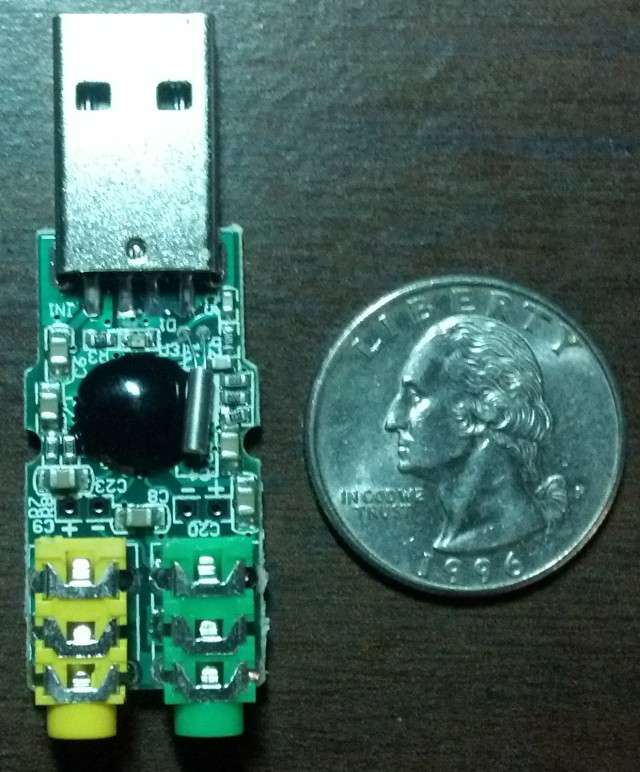
\includegraphics[scale=0.25,clip=true,trim=0 0 0 0]{portable_chapter/usb_sound_quarter.jpg} 
\caption{A USB audio device with its casing removed.}\label{fig:usb_sound}
\end{figure}

\begin{figure}[h]
\begin{verbatim}Device Drivers  --->
   <*> Sound card support  --->
      <*> Advanced Linux Sound Architecture  --->
         [*] USB sound devices  --->
            [*] USB Audio/MIDI driver\end{verbatim}
\caption{The hierarchy within the 3.8 Linux kernel \texttt{kconfig} configuration utility for enabling the USB audio device driver.  BeagleSNES now enables this driver in its BBB kernel for both HDMI and LCD3 video output.}\label{fig:kconfig_audio}
\end{figure}

The BBB only has a single USB port available.  Plugging the USB audio device into it is convenient from an implementation standpoint, but it is inconvenient because the device will extended beyond the footprint of the BBB and LCD3 cape.  Worse yet, a USB port is still needed for the USB gamepad. To resolve these issues, a small, 4-port USB hub is plugged into the single USB port and then used to provide USB to the gamepad and USB audio device.  The hub, when its casing was removed, is so small that it fits into the space between the LCD3 cape and BBB when the cape is plugged into the BBB.

Figure~\ref{fig:usb_hub} shows the positioning of the USB hub and the USB audio device when both components are positioned on top of the BBB.  The USB audio device is soldered directly to one port of the USB hub, allowing the audio jacks to be positioned in a convenient location that isn't limited by the physical position of the USB ports on the hub.  Both the hub and audio device are wrapped in electrical tape to avoid shorting and inadvertent electrical connections.  Because the LCD3 cape only uses a portion of the pins on the P8 connector, the audio jacks are positioned on the connector, next to the ethernet jack.  The assembled unit with all components is shown in Figure~\ref{fig:end_images}.

\begin{figure}[h]
\centering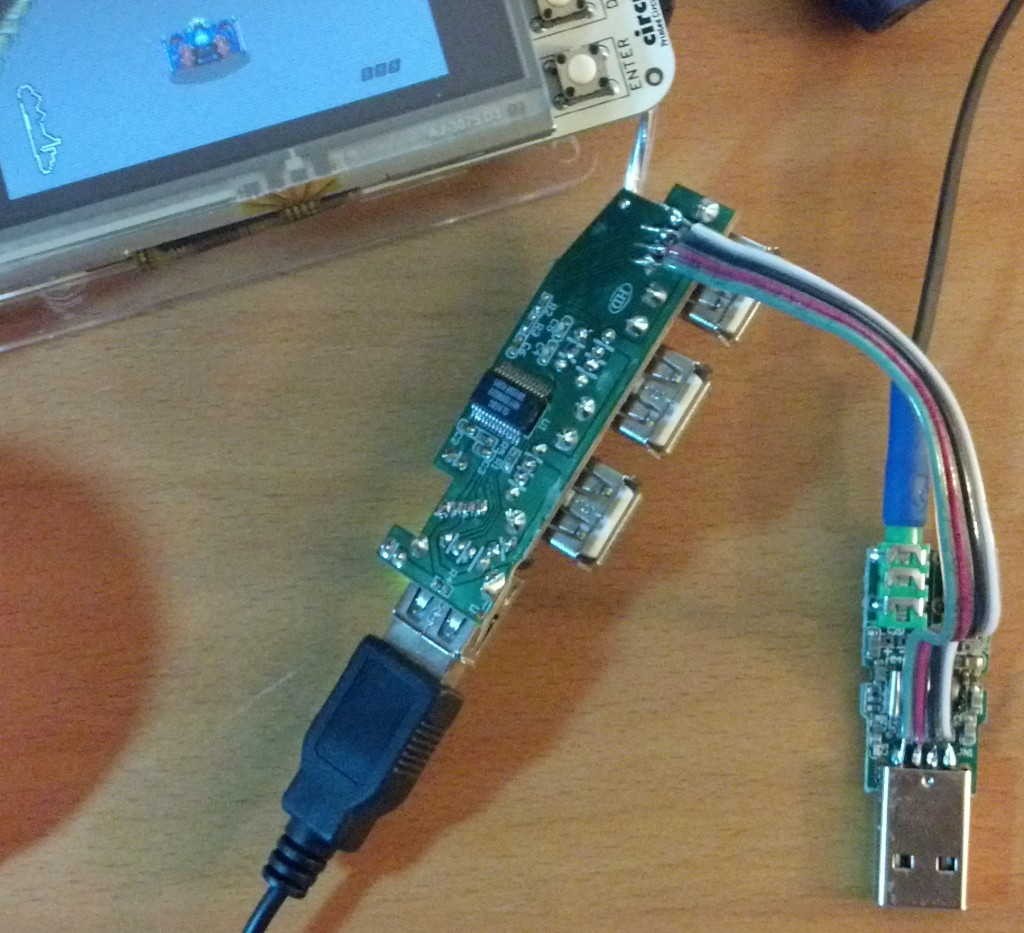
\includegraphics[scale=0.150,clip=true,trim=150 0 0 30]{portable_chapter/usb_hub_solder.jpg} 
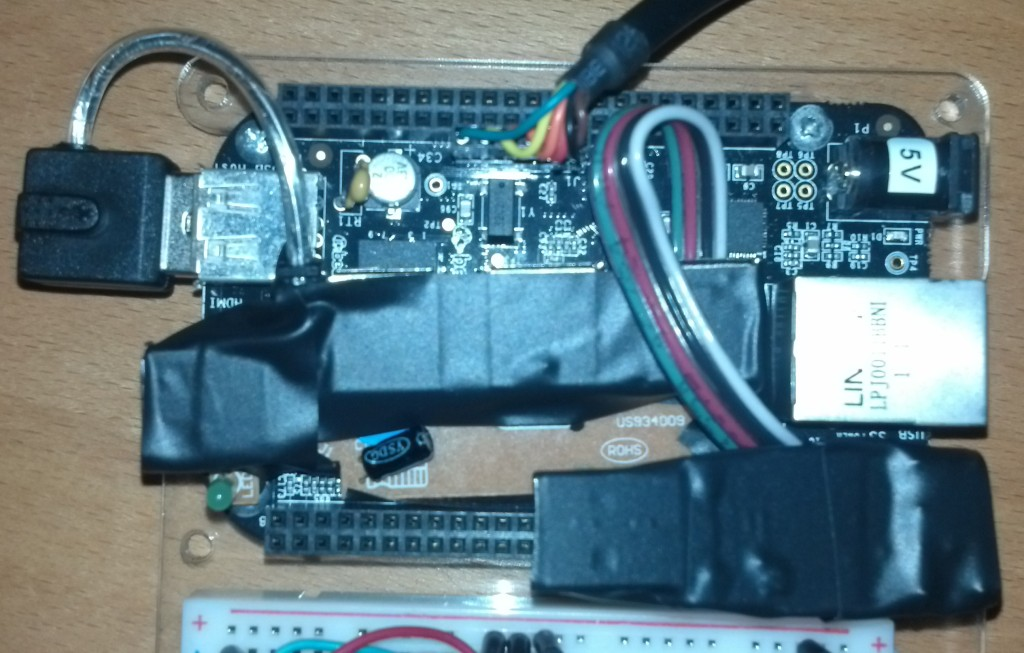
\includegraphics[scale=0.22,clip=true,trim=0 10 0 20]{portable_chapter/half_unit_tape.jpg} 
\caption{The USB hub and audio device. The audio device is soldered directly to a USB port on the hub (left).  Both the hub and device are wrapped in electrical tape and positioned on the BBB.}\label{fig:usb_hub}
\end{figure}

\begin{figure}[h]
\centering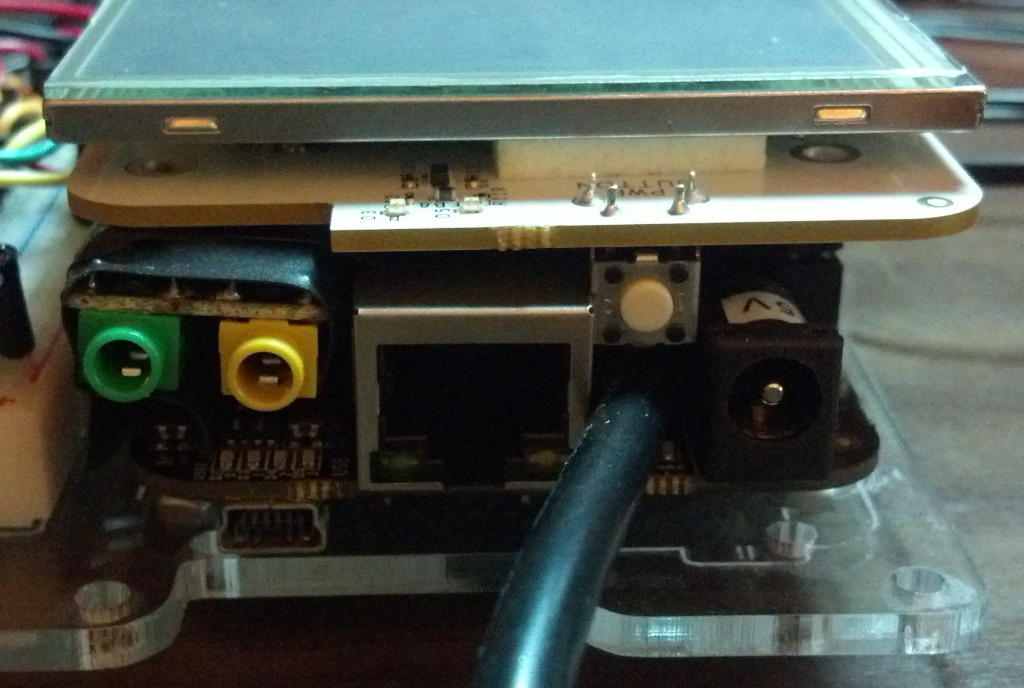
\includegraphics[scale=0.20,clip=true,trim=30 125 30 55]{portable_chapter/edge_power.jpg} 
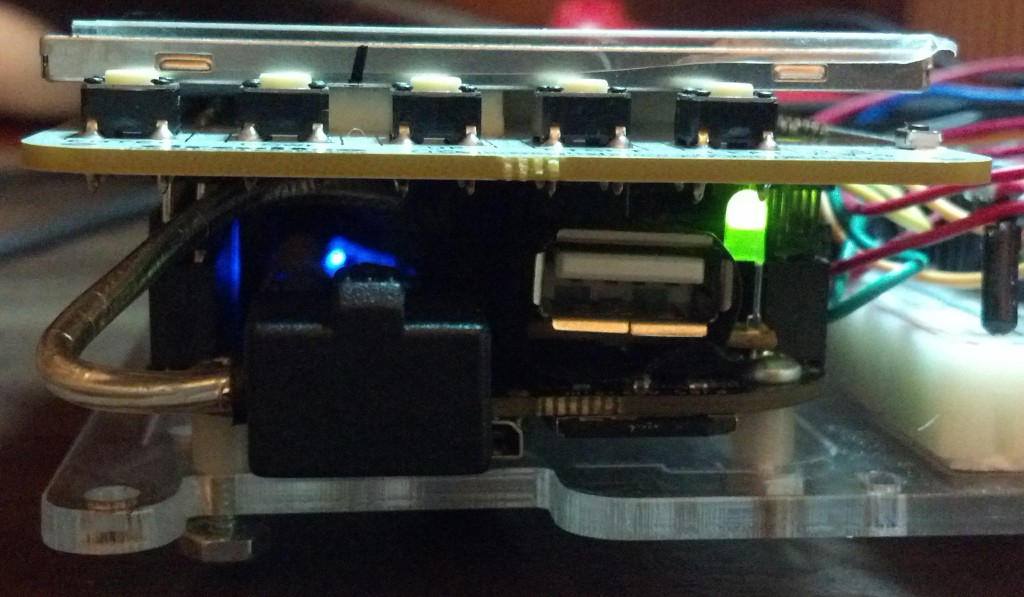
\includegraphics[scale=0.218,clip=true,trim=10 100 20 27]{portable_chapter/edge_usb.jpg} 
\caption{The assembled prototype. The edge of the unit with the power connector (left) exposes the audio jacks and the FTDI debug cable.  The edge of the unit with the BBB USB port (right) exposes the edge of the USB hub and the USB port exposed by the hub. The slight ``tilt'' of the LCD3 cape is due to the height of the FTDI debug cable preventing one side of the cape from being completely inserted.}\label{fig:end_images}
\end{figure}

\begin{updateWarn}
The CircuitCo Audio Cape requires the use of GPIO3[19], which is also used by the LCD3 cape.  So, as the moment, there is no way of using the two together.  A copy of the device tree overlay for the audio cape has been added to \texttt{/lib/firmware} so that you can experiment with the audio cape, but it won't just ``plug-and-play'' like most capes will.  You will have to manually load the overlay for the audio cape to use it.
\end{updateWarn}

\section{GPIO Input}\index{GPIO Input}\label{sec:gpio_hardware}

While requiring the user to use a USB gamepad for input is convenient for the developer, it isn't convenient for the user.  A proper implementation of a portable unit would use GPIO buttons for input and eliminate the need for the USB hub completely.  Luckily, BeagleSNES supports GPIO input.  This allows for a more elegant design for a portable platform, since a custom controller can now be built around the LCD and BBB to minimize the unit's size and weight.

By default, the GPIO support for BeagleSNES on the BBB uses all of the 13 pins on P8.7 through P8.19.  These pins are configured as input pins, and the \texttt{games.xml} file maps these pins to SNES controller events (see Section~\ref{sec:config_gpio}).  In addition, pin P8.2 is used as a ground, and pin P9.3 is used to provide 3.3V. When 3.3V is applied to a GPIO pin, a key down event is placed into the internal application event queue.  When the GPIO pin goes to ground, a key up event is triggered in the same fashion. Figure~\ref{fig:gpio_proto} shows an example implementation of GPIO input for BeagleSNES.  Each pin has a 10k ohm resistor in a pull-down configuration.

 \begin{figure}[h]
\centering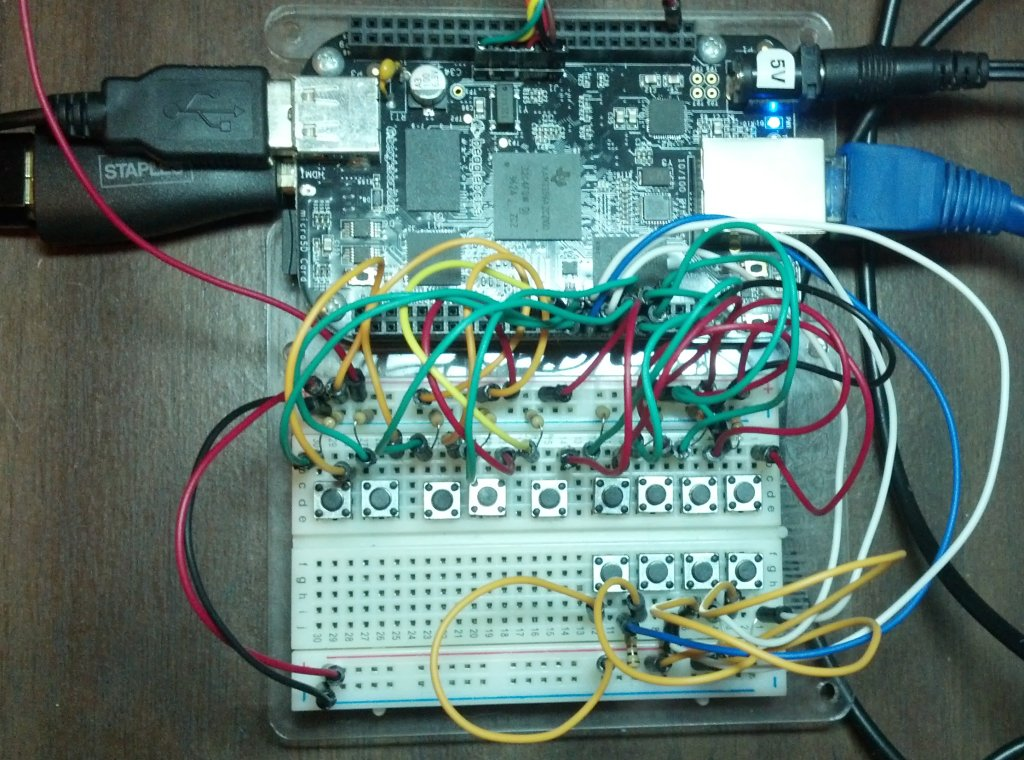
\includegraphics[angle=90,scale=0.22,clip=true,trim=50 20 0 100]{portable_chapter/gpio_proto.jpg}
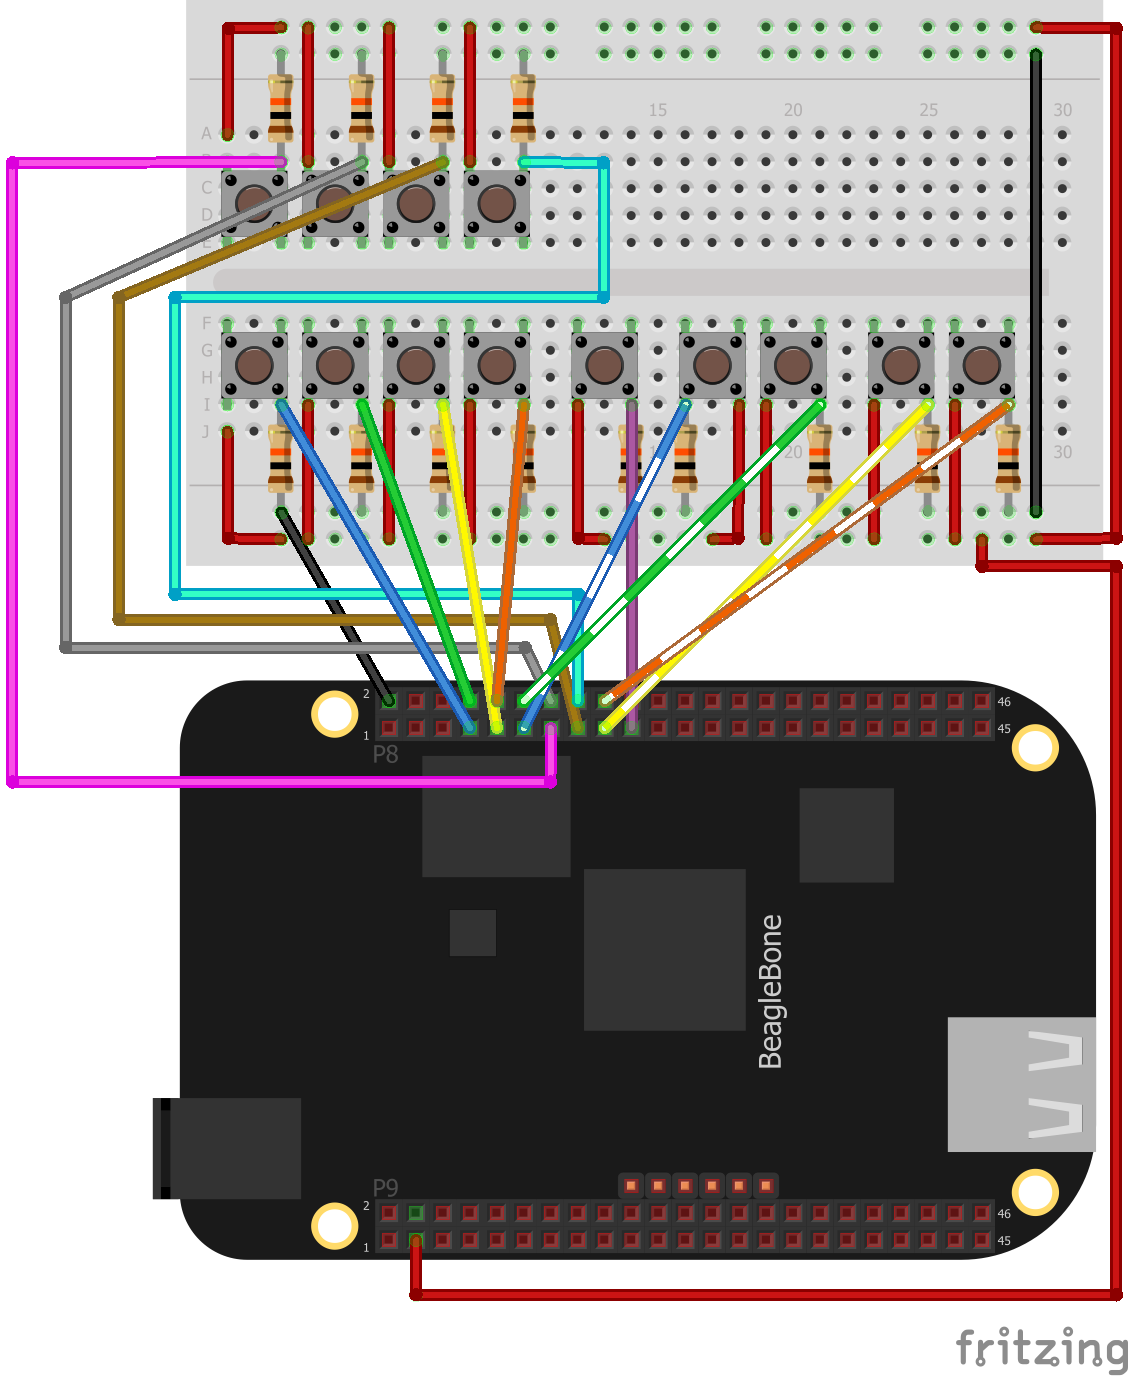
\includegraphics[scale=0.60,clip=true,trim=0 20 0 0]{portable_chapter/GPIO_bb.png}
\caption{Input via GPIO. Thirteen pins are in use in the contiguous block from P8.7 through P8.19. Each pin uses a pull-down resistor configuration. These pins implement the directional pad (4), A/B/X/Y/L/R buttons (6), start/select buttons (2), and a pause button.}\label{fig:gpio_proto}
\end{figure} 

While most of these pins can be easily accessed while the LCD3 cape is attached, pin P9.3 is used to supply power to the LCD3.  To connect to this pin, either put an intermediary ``prototyping'' cape in place that will give you access to the pin or snap a connector onto the P9.3 pin of the LCD3 cape to make a connection.  The prototype in Figure~\ref{fig:gpio_proto} used a logic analyzer probe connector to grab onto the P9.3 pin of the LCD3 cape.

\begin{updateWarn}
Always be very, very careful when working with pins on the BBB that supply voltage.  While pins P9.3 and P9.4 supply 3.3V, pins P9.5 and P9.6 supply 5V.  Connecting a 5V line to a GPIO is a sure-fire way to ruin your BBB, so always exercise caution!
\end{updateWarn}

\section{Other Considerations}\index{Other Considerations}

While the prototype is a good start, there is still work to be done in making a true "portable" system:
\begin{itemize}
\item Power is a consideration.  How much battery life will you get if the emulator is maxing out the CPU?  You'll still need a 5VDC, 2A power supply to power the board with the AM3359 running at maximum capacity.  How heavy will this battery be?  The design of the (now discontinued) CircuitCo battery cape\footnote{\texttt{http://elinux.org/CircuitCo:BeagleBone\_Battery}} might be a good reference point to start designing from.
\end{itemize}
Ultimately, it will come down to how fancy you wish to make your portable unit design and how much money you'd like to spend prototyping it.  The sky is the limit!

%----------------------------------------------------------------------------------------
%	ACKNOWLEDGEMENTS CHAPTER
%----------------------------------------------------------------------------------------

\chapter{Acknowledgements}

\section{General Acknowledgements}\index{General Acknowledgements}

While a project as complex as BeagleSNES can be organized and put together by one person, such an effort is only made possible by leveraging the hard work that others have already done.  The following people have all contributed to the pieces that make up the foundation that BeagleSNES is built upon:

\begin{itemize}
\item The team at \texttt{beagleboard.org}, who have developed the BeagleBoard family of hardware platforms.  Their efforts over the past several years have led to a variety of affordable, open-source hardware that is helping to encourage education and experience in embedded systems. 
\item Canonical (\texttt{http://www.canonical.com}), for their work on Ubuntu, which forms the base OS and file system environment of BeagleSNES.
\item Robert C. Nelson (\texttt{http://www.rcn-ee.com}), whose kernel work has formed the basis of BeagleSNES's kernel.  His wonderful Git repository of BeagleBoard kernel patches, as well as his numerous postings on various mailing lists and message boards, has provided a wealth of knowledge regarding the BB-xM platform.
\item The SDL library team (\texttt{http://www.libsdl.org}), for their on-going work in providing a straight-forward interface to the low-level multimedia systems of both desktop and embedded platforms.
\item The SNES9X team (\texttt{http://www.snes9x.com}), for their excellent, cross-platform SNES emulator. 
\item Yann Morin, for \texttt{crosstool-NG} (\texttt{http://crosstool-ng.org}), the cross-compiler toolchain-building scripts that have made the process of building a cross-compiler for BeagleSNES's development a snap. 
\item Petr Stetiar, for his \texttt{beagleboard-uboot-logo} project (\texttt{https://github.com/ynezz}) that served as a starting place for the bootloader splash screen code in BeagleSNES.
\end{itemize}

\noindent{}There is more to BeagleSNES than just code.  The following people have also provided assistance and support during the development of the project:

\begin{itemize}
\item Dave Vedder at changeMode design (\texttt{http://www.chmoddesign.com}), who developed the layout and look of the game selection menu.  If you need a GUI designed, I highly recommend him.
\item Internet Janitor and Suspicious Dish of the Something Awful forums, who have provided useful feedback pertaining to the game selection menu's fonts and animations.
\item Mathias Legrand, creator of the Legrand Orange Book LaTeX template\footnote{\texttt{http://www.latextemplates.com/template/the-legrand-orange-book}} that this document was created with.
\item Elijah Hall (\texttt{http://mrkittie.newgrounds.com}), 
\item ... Genraltweet  (\texttt{http://genraltweet.newgrounds.com}), 
\item ... conorstrejcek (\texttt{http://conorstrejcek.newgrounds.com}), 
\item ... and MarioMan94 (\texttt{http://marioman94.newgrounds.com}), the creators of several pieces of music that have served as the background audio for the BeagleSNES release video trailers.
\item Robert Beagley, who has lent his surname to the cause and who has also greatly enlightened the world at large with his many philosophical musings on bacon.
\item GameFAQS (\texttt{http://www.gamefaqs.com}), for their extensive collection of SNES game box images.
\item The EECS department at Syracuse University (\texttt{http://www.syr.edu}), who gave guidance and support to the BeagleSNES project during its initial development as a graduate course project.
\end{itemize}

\noindent{}Finally, a big thank you to Nintendo\textregistered for developing the SNES hardware platform.  Over 700+ game titles were released for the SNES\footnote{\texttt{http://en.wikipedia.org/wiki/List\_of\_Super\_Nintendo\_Entertainment\_System\_games}}, and it would be a shame if this fantastic platform faded away.

\chapterimage{Pictures/section_header.png} % Chapter heading image


%----------------------------------------------------------------------------------------
%	CHANGELOG CHAPTER
%----------------------------------------------------------------------------------------

\chapter{Project Changelog}

\section{Changelog}\index{Changelog}

\noindent{}{\bf Version 0.6 Release - 03 July 2014}

\noindent{}\emph{General:}
\begin{itemize}
\item Updated the documentation.
\end{itemize}

\noindent{}\emph{Application:}
\begin{itemize}
\item Added GPIO input support (BBB targets).
\item Added a splash screen to keep the user distracted while a background thread loads the GUI assets.
\item Added support for the pause menu with snapshot load/save.
\item Added gamepad and GPIO configuration support to the XML-based \texttt{games.xml} file.
\item Cleaned up the emulator shutdown code so that a game can be cleanly exited and control will return to the front-end GUI.
\item Changed from sync()-ing the filesystem to fsync()-ing specific files when saving snapshots, screenshots, saved games, etc.
\item Fixed hi-res blitters that were smashing the stack on some games (Donkey Kong Country, Secret of Mana, Seiken Densetsu 3).
\item Added a shrinking blitter to make the hi-res blitters work with a 320x240 display.
\item Reenabled support for loading compressed ROMs (.zip, .gz).
\item Added Expat libraries into the \texttt{configure} script.
\item Cleaned up the XML parser a bit more to eliminate closing tag errors where there weren't actually errors.
\item Added more aggressive optimization flags to the compile options to squeeze out a few more FPS. 
\end{itemize}

\noindent{}\emph{File System:}
\begin{itemize}
\item Added entries for \texttt{eth1} to \texttt{/etc/network/interfaces} for users having difficulty getting the BBB ethernet to initialize and pick up an IP via DHCP.
\item Placed a device tree overlay for the CircuitCo Audio Cape (RevB) (\texttt{BB-BONE-AUDI-02}) in \texttt{/lib/firmware} in case anyone wants to try using it with the BBB. 
\end{itemize}

\noindent{}{\bf Version 0.5 Release - 18 February 2014}

\noindent{}\emph{General:}
\begin{itemize}
\item Updated the documentation.
\end{itemize}

\noindent{}\emph{Application:}
\begin{itemize}
\item Changed the old game selection menu configuration file from \texttt{games.cfg} to the new XML-based \texttt{games.xml} format.
\item Added support for the 320x240 LCD3 display.
\item Added software volume control (mostly used by the LCD3 target).
\item Changed the name of the \texttt{snes9x-sdl.BBB} binary to \texttt{snes9x-sdl.BBB.HDMI} (for the BBB HDMI target).
\item Added the \texttt{snes9x-sdl.BBB.LCD3} binary (for the BBB LCD3 target).
\item Changed the game selection GUI to pull its button mappings from the emulator configuration file.
\item Moved the configuration, ROM, and image files to the \texttt{/boot} partition. 
\end{itemize}

\noindent{}\emph{Kernel:}
\begin{itemize}
\item Added controller driver support for ACRUX, DragonRise, GreenAsia/Pantherlord, I-Force, Sony PS3, X-Box, and ZeroPlus. 
\end{itemize}

\noindent{}\emph{Bootloader:}
\begin{itemize}
\item Updated the U-Boot bootloader for all targets to v2014.01. 
\item Modified the \texttt{setup\_BBB.sh} script so that it is now two scripts: \texttt{setup\_BBB\_HDMI.sh} (for the BBB HDMI target) and \texttt{setup\_BBB\_LCD3.sh} (for the BBB LCD3 target).
\item Setup the kernel command line arguments in the \texttt{setup\_BBB\_LCD3.sh} script to disable the HDMI cape.
\end{itemize}

\noindent{}\emph{File System:}
\begin{itemize}
\item Increased the \texttt{/boot} partition size from 64 megabytes to \textasciitilde950 megabytes.
\item Decreased the \texttt{/rootfs} partition size to fill the remainder of the 4 gigabyte microSD card image. 
\item Changed the \texttt{service.sh} script to detect whether the LCD3 cape is attached for BBB systems.
\item Modified the \texttt{/etc/modes.fb} file to include a 320x240 mode for the new LCD3 display target.
\item Added the Expat 2.1.0 library and headers to \texttt{/usr/local}.
\end{itemize}

\noindent{}{\bf Version 0.4 Release - 07 June 2013}

\noindent{}\emph{General:}
\begin{itemize}
\item Reduced boot time from 20 seconds down to about 10-12 seconds in "fast boot" mode.
\item Updated the documentation.
\end{itemize}

\noindent{}\emph{Application:}
\begin{itemize}
\item Added support for two gamepads via an external USB hub (BBB).
\item Added support for an arbitrary number of games to be listed in the game selection menu.
\item Removed the user space workaround that adds USB hotplugging (BBB).
\end{itemize}

\noindent{}\emph{Kernel:}
\begin{itemize}
\item Updated the kernel tree from 3.8.11 to 3.8.13 (BBB).
\item Patched the kernel to fix issues with USB hotplugging and "babble interrupts" (BBB).
\end{itemize}

\noindent{}\emph{Bootloader:}
\begin{itemize}
\item Added the kernel command line \texttt{init=} option in \texttt{uEnv.txt} to use \texttt{init.sh} as the \texttt{init} process of the system for "fast boot" mode.
\end{itemize}

\noindent{}\emph{File System:}
\begin{itemize}
\item Added the \texttt{init.sh} script to act as the new \texttt{init} process of the system.
\item Modified \texttt{init.sh} to mount various file systems, start the \texttt{udevd} daemon, and launch BeagleSNES's \texttt{service.sh} script.
\end{itemize}

\noindent{}{\bf Version 0.3 Release - 17 May 2013}

\noindent{}\emph{General:}
\begin{itemize}
\item Added support for the BeagleBone Black platform.
\item Added \texttt{setup\_BBB.sh} and \texttt{setup\_BBxM.sh} scripts in the boot partition to switch the full system image from BBB to BB-xM and back.
\item Made BBB the default state of the full system image.
\item Updated the documentation.
\end{itemize}

\noindent{}\emph{Application:}
\begin{itemize}
\item Modified the graphics to support 720x480 (BBB) and 640x480 (BB-xM) based upon preprocessor defines.
\item Added support the dynamic plugging/unplugging of gamepads for BBB.
\item Fixed a timing bug where the selection GUI might freeze.
\item Fixed a bug where SRAM (saved games) was not being written out to the microSD card. Also added a \texttt{sync()} call on SRAM activity to ensure saved games are stored on the microSD card.
\item Modified the \texttt{service.sh} launch script to detect whether the system is BBB or BB-xM and launch the appropriate binary.
\end{itemize}

\noindent{}\emph{Kernel:}
\begin{itemize}
\item Added a new Linux kernel tree (3.8.11) to support the BBB.  The BB-xM is still using the 3.7.10 kernel tree.
\item Added a 720x480 kernel splash screen for the BBB port.
\end{itemize}

\noindent{}\emph{Bootloader:}
\begin{itemize}
\item U-boot has been upgraded from v2013.01 to v2013.04.
\item The \texttt{beaglesnes\_build.sh} build script has been changed to have an additional configuration target for the BBB.
\end{itemize}

\noindent{}\emph{File System:}
\begin{itemize}
\item Both the BBxM and BBB kernels are in the \texttt{/boot} partition.  \texttt{BBB} and \texttt{BBxM} subdirectories were added to hold platform-specific bootloader and \texttt{uEnv.txt} files.
\end{itemize}

\noindent{}{\bf Version 0.2 Release - 23 April 2013}

\noindent{}\emph{General:}
\begin{itemize}
\item Changed from analog video (S-Video) to digital video (DVI).
\item Decreased boot time from about 25 seconds down to about 20 seconds.
\item Improved gamepad support.
\item Added a kernel splash screen.
\item Published the first version of this documentation!
\end{itemize}

\noindent{}\emph{Application:}
\begin{itemize}
\item Changed resolution of game selection menu from 720x482 to 640x480.
\item Changed resolution of emulator from 616x478 to 640x480.
\item Added support the dynamic plugging/unplugging of gamepads.
\item Removed several checks for movie playback and saved states from main emulation loop.
\item Changed the internal emulator scaling algorithm from "Simple2x1" to "Smooth2x2" to accommodate for the increased sharpness of the digital video signal. 
\item Moved the loading of background music and the rendering of dynamic text so that they occur after the BeagleSNES logo and gradient bar are loaded and rendered to the screen.  This gets \emph{something} up on the screen ASAP for the end-user.
\end{itemize}
\noindent{}\emph{Kernel:}
\begin{itemize}
\item Removed video encoder (VENC) support (S-Video support removed).
\item Added parallel display interface (DPI) support, generic DPI panel driver, and TFP410 DPI-to-DVI chip driver (DVI support added).
\item Built SMC9XXX network support directly into the kernel, rather than as a module.  Now no kernel modules are dynamically loaded.
\item Added a 640x480 splash screen displayed during kernel bootstrapping by replacing the 80x80 tux boot icon with the splash image.
\item Removed a bunch of device driver modules from the build, since they weren't actually being used anymore.
\end{itemize}
\noindent{}\emph{Bootloader:}
\begin{itemize}
\item Preliminary support for a bootloader splash screen was added (\texttt{dss\_init()} in \texttt{beagle.c}).
\item Changed \texttt{mpurate} from \texttt{auto} to \texttt{800} in \texttt{uEnv.txt} to force the kernel to set the clock to 800 MHz immediately, rather than wait for the governor to adjust it.
\item Cleaned up a bad PLL4 clock register setting that was preventing logging in through the debug serial output (\texttt{beagle.c}). 
\item Changed the video configuration in \texttt{uEnv.txt} to use digital 640x480@60 Hz (DVI) instead of analog 720x482@30 Hz (NTSC).
\end{itemize}
\noindent{}\emph{File System:}
\begin{itemize}
\item The \texttt{service.sh} launch script for the BeagleSNES application is now started via the script \texttt{/etc/rc.local}, rather than as an "at reboot" \texttt{cron} job in \texttt{crontab}.  This gets the game selection menu up and available much quicker (prior to \texttt{tty} initilization).
\item The \texttt{loadcpufreq}, \texttt{cpufrequtils}, and \texttt{ondemand} services were removed from all \texttt{/etc/rc?.d} directories.
\item The rootfs file system was shrunk down from 7.5 gigabytes to 3.5 gigabytes.
\end{itemize}
\noindent{}{\bf Initial Release - 15 March 2013}
\begin{itemize}
\item Registered the \texttt{beaglesnes.org} domain name.
\item Created the BeagleSNES SourceForge project.
\item Created the project launch trailer video.
\item Cleaned up the files and made them available on the web.
\end{itemize}
\end{document}
